%% Template for a preprint Letter or Article for submission
%% to the journal Nature.
%% Written by Peter Czoschke, 26 February 2004
%%

\documentclass{nature}
%\documentclass[12pt]{article}

%% make sure you have the nature.cls and naturemag.bst files where
%% LaTeX can find them

\bibliographystyle{naturemag}

\usepackage{graphicx}
\usepackage{amssymb,amsfonts,amsmath}
\usepackage{subfigure}
\usepackage{stfloats}


%% OPTIONAL MACRO DEFINITIONS
\def\s{\sigma}
\newcommand{\be}[0]{\begin{equation}}
\newcommand{\ee}[0]{\end{equation}}
\newcommand{\lb}[0]{\left(}
\newcommand{\rb}[0]{\right)}

\usepackage[modulo]{lineno}
\linenumbers

\title{Arctic sea ice loss and Eurasian surface air temperature from 1979-2012}
%\title{Arctic sea ice loss and Eurasian surface air temperature on a multi-decadal timescale}
%\title{Arctic sea-ice loss and the multi-decadal decrease of Eurasian surface air temperatures} %87 char
%\title{Arctic sea-ice loss and cold Eurasian winters in the face of internal variability}% 81char

%% Notice placement of commas and superscripts and use of &
%% in the author list


\author{Kelly E. McCusker,*$^{1,2}$ \& John C. Fyfe,$^{2}$ \& Michael Sigmond$^2$}

% NatGeo requirements:
% Title If possible, the title should give a sense of the main new finding, and should not exceed 90 characters, including spaces. Nature Geoscience titles do not contain technical terms or abbreviations unless absolutely necessary. We strongly discourage punctuation or active verbs.@@
% Letter 2,000 words no methods, 3 figures
% Article 3,000 words no methods, include section titles, 6 figures. No refs in abstract. ~500 words of Intro. 1-2 para of conclusions


\begin{document}

\maketitle

\begin{affiliations}
 \item School of Earth and Ocean Sciences, University of Victoria, Victoria, BC, V8P 5C2, Canada
 \item Canadian Centre for Climate Modelling and Analysis, Environment Canada, Victoria, BC V8W 2Y2, Canada
\end{affiliations}


\begin{abstract}
%Arctic sea ice loss has been implicated in the recent trend toward unusually cold Eurasian winters \cite{liu12,mori14,kim14}. Whether the linkage follows from anthropogenic sea ice loss, however, remains an open question as the sea-ice loss combines anthropogenic response and internal (random) variability \cite{swart15,wettstein14} and because of confounding wintertime variability over the Eurasian continent \cite{deser12b,screen14a}. Here, we isolate the anthropogenic and random components of the linkage using a large ensemble of atmosphere-only model simulations with prescribed sea ice loss taken from simulations of the companion atmosphere-ocean-cryosphere model and from observations. We find no evidence of a sea-ice loss related decrease in Eurasian winter temperature. However, we do find long periods of winter Eurasian cooling linked to internally-generated circulation features over the Barents and Kara Seas regions of the Arctic. These results challenge the perception that Arctic sea ice loss was responsible for the recent prevalence of unusually cold Eurasian winters, showing instead that these winters were more likely the consequence of internal variability, with implications for our understanding of impacts and adaptation in human and natural high-northern latitude systems. 
Arctic sea ice concentration has declined in all seasons since satellite observations began in 1979 \cite{simmonds15}. At the same time and in spite of significant hemispheric warming in boreal winter that is in large part anthropogenic \cite{gillett08,qian15}, Eurasian surface air temperature has decreased. Previous studies have suggested that Eurasian surface air temperature in boreal winter is sensitive to changes in Arctic sea ice, and that recent, cold winters were fundamentally caused by the loss of ice \cite{honda09,liu12,outten12,inoue12,mori14,kim14}. Here we show, using a large ensemble of atmosphere-ocean-cryosphere model simulations and a large ensemble of simulations from the companion atmosphere-only model in which the response to sea ice loss is isolated, that a decline in Arctic sea ice does not systematically lead to a decrease in Eurasian wintertime surface air temperature. Instead, long term decreases in Eurasian wintertime surface air temperature are associated with internally-generated height anomalies over the Barents and Kara Seas. These results suggest that Arctic sea ice loss is not responsible for the cooling over Eurasia in recent decades, but that it is more likely the consequence of internal variability, with implications for our understanding of impacts and adaptation in human and natural high-northern latitude systems. %circulation features that include positive geopotential

%Arctic sea ice loss, particularly in the Barents and Kara Seas, has been implicated in the recent trend toward unusually cold Eurasian winters \cite{honda09,liu12,outten12,inoue12,mori14,kim14}. However, observational evidence of the direction of causation remains inconclusive \cite{sorokina15}, and modelling evidence yields variable results \cite{honda09,gerber14} in part due to large atmospheric internal variability in sea ice loss \cite{swart15,wettstein14} and confounding wintertime variability over the Eurasian continent \cite{deser12b,screen14a}. Eurasia has also experienced a long term (1979-2012) wintertime cooling trend that deviates significantly from general hemispheric warming. Here we investigate whether long-term sea ice decline is linked with Eurasian cooling on a multi-decadal timescale using a large ensemble of atmosphere-ocean-cryosphere model simulations, and further isolate the influence of sea ice loss on this linkage using a large ensemble of simulations from the companion atmosphere-only model with prescribed sea ice loss taken from the atmosphere-ocean-cryosphere model. We find that sea ice loss contributes to an anomalous anti-cyclone over the Barents and Kara Seas in winter, however it does not systematically lead to a decrease in Eurasian wintertime surface air temperature. Instead, long term decreases in Eurasian wintertime surface air temperature are associated with internally-generated circulation features that include positive geopotential height anomalies over the Barents and Kara Seas. These results suggest that Arctic sea ice loss is not responsible for the lack of significant warming over Eurasia, but that it is more likely the consequence of internal variability, with implications for our understanding of impacts and adaptation in human and natural high-northern latitude systems. % (@@and from observations)

\end{abstract}

Global average surface air temperatures in the boreal cold season have been rising faster than the long-term annual average \cite{wallace12} and exhibit further enhanced warming over the Arctic in part due to positive feedbacks related to sea-ice loss \cite{screen10,cohen14}. Epoch differences of winter (December-January-February; DJF) surface air temperature (SAT) between 2002-12 and 1979-89 reveal warming upward of 2$^\circ$C over the polar cap, collocated with areas of sea ice loss (Figure \ref{fig:fig1}a). Contemporaneous cooling of greater than 1$^\circ$C over parts of the Eurasian continent in winter is also evident. Since 1979, Eurasian SAT in winter has deviated substantially from hemispheric warming (Figure \ref{fig:fig1}b), which is partly attributable to anthropogenic forcing \cite{gillett08,qian15}. Eurasian SAT has decreased 0.4$^\circ$C between these two time periods against significant ($p<$0.01)  Northern hemisphere warming of 0.5$^\circ$C, a total deviation of -0.9$^\circ$C. Coincident with this decrease in winter SAT, large reductions in autumn and winter Arctic sea ice area have occurred \cite{simmonds15}, particularly in the Barents and Kara Seas (BKS) sector where a statistically significant decrease in winter sea ice area between epochs (-0.3e$^6$ km$^2$; $p<$0.001) is observed (Figure \ref{fig:fig1}c). %stroeve12,

%The evolution of Eurasian SAT with northern hemisphere SAT removed illuminates the substantial deviation SAT has taken from expected hemispheric warming (Figure \ref{fig:fig1}b). The difference between epochs marked in gray shading in Figure \ref{fig:fig1}b equals -0.9$^\circ$, a substantial deviation from the expected general hemispheric warming of 0.5$^\circ$C ($p<$0.01). %This feature is particularly striking when considered in the context of broad hemispheric warming that is partly attributable to anthropogenic forcing \cite{gillett08,qian15}.

% null is that the SAT should be significantly warming. then test 2002-12 > 1979-89 (pval/2)

%Long term trends in atmospheric circulation 
% , and is linked to a trend in the pattern of geopotential height
%  and linked to cold-air advection brought about by an increasing trend in 
%; a feature that is particularly striking when considered in the context of broad hemispheric warming, which can in part be attributed to anthropogenic forcing \cite{gillett08,qian15}. The evolution of Eurasian winter SAT shows a substantial deviation from expected general hemispheric warming
%with northern hemisphere average SAT removed shows a substantial deviation from the expected general hemispheric warming
%@@ could also estimate "externally forced" trend with CanESM2
%Since the year 2000, Eurasian winters have tended toward increasingly cold anomalies, especially in relation to the evolution of northern hemisphere temperature; Figure \ref{fig:fig1}b shows the evolution of Eurasian winter SAT with northern hemisphere average SAT removed. The difference of this measure of Eurasian SAT between epochs marked in gray shading in Figure \ref{fig:fig1}b equals -0.9$^\circ$, a substantial deviation from the expected general hemispheric warming of 0.5$^\circ$C ($p<$0.01). Coincident with this decrease in winter SAT, large reductions in autumn and winter Arctic sea ice area have occurred \cite{stroeve12}, particularly in the Barents and Kara Seas (BKS) sector where a statistically significant decrease in sea ice area between epochs (-0.3e$^6$ km$^2$; p$<$0.001) is observed (Figure \ref{fig:fig1}c).

%-1.1$^\circ$C, and indicates Eurasian SAT has deviated a significant amount from expected general hemispheric warming (p=0.09). Coincident with this decrease in winter SAT, large reductions in autumn and winter Arctic sea ice area have occurred \cite{stroeve12}, particularly in the Barents and Kara Seas (BKS) sector where a statistically significant decrease in sea ice area between epochs (-0.3e$^6$ km$^2$; p$<$0.001) is observed (Figure \ref{fig:fig1}c). %@@ what is the p val of raw SAT diff?
% SAT eurasiamori avg and DJF avg trend (1979-01-01,2014-12-31) pval: 0.303827136006
% SAT eurasiamori avg and DJF avg trend (2000-01-01,2014-12-31) pval: 0.107588506299

%1979-01-01,1989-12-31 2002-01-01,2012-12-31 MATCHES BOUNDARY CONDITIONS 
%EPOCH diffs for eurasiamori DJF avg pval: 0.602542449647
%  --- mean val: -0.402862777711
%EPOCH diffs for eurasiamori DJF-NH: avg pval: 0.193536402555
%  --- mean val: -0.877272681435
%EPOCH diffs for SIC bksmori DJF avg pval: 0.000790793963746
%  --- mean val: -0.0614791972683
%EPOCH diffs for SIA bksmori DJF avg pval: 0.000790793963746
%  --- mean val: -250793697783.0 (this is -0.25e12)


% In an email dated 5/25/2015 from Fyfe: In the text we can note that the epoch T difference is -1.1 C (different from 0 at p = 0.09). The epoch SIA differences is -0.3 (different from zero at p = 0.0003).
%    See below for the values that match John's calcs -- it's the timesel 
% 1979-01-01,1989-12-31 2002-01-01,2013-12-31
%EPOCH diffs for eurasiamori DJF avg pval: 0.485527295537
%  --- mean val: -0.521729410085
%EPOCH diffs for eurasiamori DJF-NH: avg pval: 0.134284782073
%  --- mean val: -0.981054320546
%EPOCH diffs for SIC bksmori DJF avg pval: 0.000390644676974
%  --- mean val: -0.0667587284786
%EPOCH diffs for SIA bksmori DJF avg pval: 0.000390644676974
%  --- mean val: -272330627569.0

%% 1979-01-01,1990-12-31 2002-01-01,2013-12-31
%EPOCH diffs for eurasiamori DJF avg pval: 0.371152330367
%  --- mean val: -0.648778655157
%EPOCH diffs for eurasiamori DJF-NH: avg pval: 0.0913761235493
%  --- mean val: -1.06966767897
%EPOCH diffs for SIC bksmori DJF avg pval: 0.000323289685762
%  --- mean val: -0.0646821380456
%EPOCH diffs for SIA bksmori DJF avg pval: 0.000323289685762
%  --- mean val: -263859537889.0

%\cite{honda09,liu12,outten12,inoue12,mori14,kim14}.
Observationally-based studies confirm a positive correlation exists between Barents/Kara Seas sea ice concentration (SIC) and Eurasian SAT \cite{inoue12,outten12,sato14,sorokina15}, yet the direction of causality is unclear. Some implicate the sea ice loss in the Barents/Kara in initiating Eurasian cooling through a weakened meridional temperature gradient and ensuing changes in circulation and cyclone track \cite{inoue12,outten12}, while others suggest atmospheric circulation variability, not sea ice loss, drives both \cite{sato14,sorokina15}. A similar lack of clarity is evident in modelling results in which the influence of a change in sea ice is isolated. There is support for the hypothesis that Barents/Kara sea ice loss can initiate more frequent or more intense cold Eurasian SAT anomalies through a Rossby wave-train emanating out of the Barents/Kara Seas region incited by turbulent heat flux from increased areas of open water \cite{honda09,petoukhov10,mori14,kim14,peings14,gerber14}. The magnitude of this modelled effect is typically weak, and the timing and placement of decreased SAT is not consistent. Others suggest the root cause of both Barents/Kara sea ice loss and Eurasian cooling is a third factor \cite{sato14,peings14b}, or find no detectable signal in SAT outside of the Arctic \cite{screen14a}. It thus remains unclear as to the role, if any, changes in SIC play in Eurasian temperature trends. Here we evaluate the likelihood of a long term (1979-2012) Eurasian cooling event on the order of that observed, and further address whether a concurrent decrease of winter Barents/Kara SIC could be the cause of such a decrease in Eurasian winter SAT. %Clarification of the link between sea ice loss in the Barents/Kara Seas and Eurasian SAT is warranted. %Furthermore, the potential linkages found in these studies generally apply on intra-seasonal to interannual timescales. %@@@ say something about positive Z500 %This may relate to differences in model used, or in experimental design. Yet still % using a large ensemble of coupled historical simulations

%Similarly, modelling studies diverge on the role of BKS sea ice loss in Eurasian wintertime SAT. Some previous modelling studies in which the influence of a change in sea ice is isolated provide support for the hypothesis that BKS sea ice loss can initiate Eurasian cooling through a Rossby wave-train emanating out of the BKS region, incited by turbulent heat flux from the increased area of open water \cite{honda09,petoukhov10,mori14,kim14,peings14}. However, the magnitude of the modelled effect is weak compared to the observed Eurasian cooling, and the timing and placement of the cold anomaly is not consistent. Furthermore, still other studies point to sea surface temperature (SST) changes in the North Atlantic or @@ as a possible root sources of Rossby wave propagation and Eurasian cooling (cite@@). 

%Further clarification of the link between sea ice loss in the Barents-Kara Seas and Eurasian SAT anomalies is thus warranted. Here we evaluate the likelihood of a long term (1979-2012) Eurasian cooling event on the order of that observed using a large ensemble of coupled historical simulations, and further address whether or not a multi-decadal decrease of Barents-Kara sea ice concentration in winter is not only associated with, but could be the cause of a decrease in Eurasian winter SAT over this time period. % However, the observed relationship of BKS turbulent heat flux to Eurasian SAT suggests atmospheric variability, not sea ice loss, drives both \cite{sorokina15}. %there have been a greater number of Eurasian winters exhibiting increasingly cold anomalies, % along the western half of the Russian coastline  % The epoch difference in BKS sea-ice area (SIA; -0.3e$^6$ km$^2$) is also statistically significant (p$<$0.001).

%Here we address whether a long term (1979 - 2012) decrease of Barents-Kara sea ice concentration in winter is not only associated with, but could be the cause of a decrease in Eurasian winter SAT over this time period. % (Figure \ref{fig:fig1}). %We take into account the powerful influence of internal variability of the climate system, as well as the imprint of internal variability on the change in sea ice itself.  % @@The general hypothesis is that a decrease in sea ice concentration initiates local warming that leads to changes in circulation that cause Eurasian wintertime cooling (@@cite). 

%Few studies have addressed whether the long term trend in Arctic or Barents-Kara sea ice concentration has influenced the significant trend in Eurasian winter SAT. @@

We do this by analysing changes in SIC and SAT in coupled simulations and in atmosphere-only simulations with prescribed sea ice loss. The coupled simulations consist of a fifty-member large ensemble (LE) of Canadian Earth System Model version 2 (CanESM2 \cite{arora11}) simulations with historical forcing. Each CanESM2 realization is executed with identical historical forcings with slightly varied initial conditions. As such, we are able to characterize the impact of external forcing and internal variability on changes in Barents/Kara SIC, Eurasian SAT, and their relationship over the decades since 1979. The historical LE results are presented as epoch differences between 2002-12 and 1979-89 DJF averages for each realization, which we refer to collectively as ``CGCM". The average of CGCM, in which internal variability has been averaged out, represents the response due to external forcings. The externally-forced response of DJF SIC in the Barents/Kara Seas is a decrease in SIC of 5.8\% in absolute terms, with a spread of nearly 13\%, including 2 members with sea ice growth (Figure \ref{fig:fig2}a), consistent with a significant role for internal variability on sea ice even on timescales greater than 30 years \cite{swart15}. Observed sea ice loss (-6.2\%), derived from satellite measurements by the National Snow and Ice Data Center (NSIDC; see Methods), is comparable to the externally-forced value in this sector, and is consistent with the presence of a human influence on Arctic sea ice \cite{min08}. The corresponding forced response of Eurasian SAT in winter is a warming of 1.31$^\circ$C, with positive anomalies making up the vast majority of the changes in Eurasian SAT in CGCM (Figure \ref{fig:fig2}b). Just 2 of 50 ensemble members show a decrease in SAT, and only one is comparable to the observed value of -0.40$^\circ$C, equalling -0.34$^\circ$C. The observed change in boreal winter Eurasian SAT is thus exceptional in the context of multiple realizations of the response to historical forcings, while the observed change in Barents/Kara SIC is comparable to the forced change. Therefore, factors other than sea ice loss are necessary to explain the observed Eurasian cooling. Yet the question remains as to whether Arctic sea ice loss may have contributed to this decrease in SAT.

% The probability of a negative change in SAT is just p=0.04. In comparison, observed cooling over this time period equals -0.40$^\circ$C, slightly colder than the coldest member of CGCM (-0.34$^\circ$C).  % The response of DJF sea ice concentration in the Barents/Kara Seas to external forcing is represented by the CGCM average change over this time period and is equal to -5.8\% (Figure \ref{fig:fig2}a). This value is comparable to observed loss in this sector (-6.2\%) derived from satellite measurements by the National Snow and Ice Data Center (NSIDC; see Methods), and consistent with the presence of a human influence on Arctic sea ice \cite{min08}. However, observations represent just one potential reality due to internal variability; internal variability in CGCM produces a range of anomalies that span nearly 13\% in this region in winter --- even on a multi-decadal timescale --- including two ensemble members with positive anomalies. 

%, the question remains: Does this change in sea ice play a role in setting Eurasian SAT? %In order to determine what role, if any, Arctic sea ice changes have in setting %Does Arctic sea ice loss play a role in  Therefore, factors other than sea ice loss are necessary to explain the observed anomalous cooling. We first isolate the influence of sea ice  %Despite the requirement of external factors to explain the observed cooling, it is possible that sea ice loss has played a role through mechanisms 
%Therefore, factors other than changes in sea ice loss are necessary to explain the observed anomalous cooling, but could sea ice loss have played a role? @@ % Thus, Eurasian SAT is dominated by anthropogenic forcing in CGCM, with a rare occurrence of a long-term cooling trend. @@reword or clarify next sentence@@ This is the case despite the CGCM average decrease in Barents/Kara sea ice concentration being comparable in magnitude to that of observations.
%having average sea ice loss in the Barents/Kara seas comparable in magnitude to observations. % However, is it possible that changes in sea ice play a role in modulating Eurasian SAT? % a probability of cooling of just p=@@. % , as seen in the average of CGCM Eurasian SAT anomalies

%The change in September and DJF sea ice area over the whole of the Arctic over this time period compares well with NSIDC (Supplementary Figure @@), lending additional credence to the use of this climate model for our study.  % The favourable comparison of the CanESM2 historical simulations to observations indicates that CanESM2 is an appropriate tool to investigate the atmospheric response to sea ice

%, while the preindustrial control is segmented into 11-year climatologies and randomly sampled to generate a set of fifty anomalies, which we refer to as ``Preindustrial" (see Methods).  % as well as a 1,000 year CanESM2 preindustrial control simulation with no forcing % In comparison, the relationships uncovered in the preindustrial simulation are due only to internal variability.
%We start by examining the first link in the chain, the change in Arctic SIA. The average DJF Arctic SIA anomaly in Preindustrial is approximately zero, whereas it is -1.2 million km$^2$ in CGCM due primarily to anthropogenic forcing over this time period. Yet, even on this multi-decadal timescale, internal variability produces a range of anomalies that span nearly one million km$^2$ in CGCM and over one million km$^2$ in Preindustrial (Supplementary Figure \ref{fig:supfig1}), consistent with previous findings \cite{swart15}. The observed value (-0.78 million km$^2$), derived from satellite measurements by the National Snow and Ice Data Center (NSIDC), is encompassed only by the 2.5-97.5\% range of CGCM anomalies and not by Preindustrial anomalies, consistent with the presence of a human influence on observed sea ice loss \cite{min08}. 

To isolate the impact of Arctic sea ice loss on Eurasian SAT, we execute pairs of 120-year atmosphere-only ``time-slice" simulations with prescribed ``past" (1979-89) and ``present day" (2002-12) SIC, sea surface temperature (SST), and sea ice thickness (SIT) taken from five members of CGCM. The AGCM experiments are constructed such that the only changes between past and present day are Arctic SIC, SIT, and SST where SIC $<$ 10\% in the present day but not in the past (see Methods). The choice to use model output as boundary conditions was made so that all surface forcings are physically consistent, so that multiple forcing patterns can be tested, and so that atmosphere-only results can be cleanly compared to their fully coupled counterparts. The prescribed SIC anomalies averaged in the Barents/Kara Seas in DJF are shown as gray circles in Figure \ref{fig:fig2}a. The atmosphere-only results, which we refer to as ``AGCM", are presented as anomalies between present-day and past simulations, and are sub-sampled into fifty 11-year averages to mirror the sampling uncertainty of CGCM. %Thus, AGCM\_variable anomalies are due to the loss of Arctic sea ice, and to uncertainty due to atmospheric internal variability. %Eurasian SAT anomalies in CGCM are due to a convolution of external forcing, internal variability, and coupled feedbacks in the climate system. 

We find that Arctic sea ice loss in isolation does not cause a systematic Eurasian winter cooling (Figure \ref{fig:fig3}); the average change in Eurasian SAT in AGCM is 0.09$^\circ$C, with 50\% of anomalies falling below zero and 50\% above. Moreover, changes in Eurasian SAT show no preference for cooling in an additional pair of 120-year time-slice simulations with boundary conditions computed from observed SIC (``AGCM\_obs"; see Methods). Just 3 of 7 eleven-year anomaly periods show a decrease in SAT. These findings indicate that while Eurasian cooling can occur and appear to be caused by sea ice loss, it is equally likely that warming can occur. Furthermore, changes in Eurasian SAT in boreal winter in AGCM are indistinguishable from those changes in a long Preindustrial control simulation that is treated in a similar manner to retain the same sampling uncertainty as CGCM and AGCM (see Methods and Supplementary Figure S1). Thus, by this measure, the fluctuations in SAT changes in AGCM are indistinguishable from variations in Eurasian SAT changes that are dictated by internal variability, in accordance with evidence that the sphere of influence of sea ice does not robustly reach the mid-latitudes \cite{screen14a}. %Thus, there is nothing special about the pattern of observed sea ice loss.

%Finally, to test whether the pattern of sea ice change in observations is particularly special and produces a stronger change in Z500 and Eurasian cooling, we execute one additional pair of 120-year time-slice simulations with boundary conditions computed from NSIDC SIC (see Methods). Here again there is no systematic Eurasian cooling --- just 3 of 7 eleven-year anomaly periods show a decrease in SAT --- and these periods of decreased SAT are instead associated with internally-generated circulation features. 

  %(@@test the shortterm distributions against e/o (AGCM/AGCMfixed/PreI), add the box at top for AGCM\_fixed?) % [@@long-term averaging here?]  % Moreover, Eurasian SAT shows nearly identical behaviour in an additional atmosphere-only ensemble of time-slice simulations in which the prescribed sea ice anomalies equal the average of the 5 boundary conditions in AGCM\_variable, and are held fixed for 600 years of simulations (``AGCM\_fixed"; see Methods). The distribution of DJF Eurasian SAT anomalies in AGCM\_fixed is not statistically different from that of AGCM\_variable, with an average SAT change of 0.005$^\circ$C, and equal probability of negative and positive anomalies.

%These SAT anomaly distributions are similar to that of Preindustrial, indicating that the multi-decadal SAT variations in AGCM are simply dictated by internal variability.   %what would be expected of Eurasian SAT due solely to internal variability in an unforced simulation %The influence of the differences in the sea ice boundary conditions is indistinguishable from internal variability (Supplementary Information) and so we do not attempt to separate their contributions further.

To understand what drives Eurasian SAT, if not sea ice, we turn to the large-scale circulation --- which has a significant impact on mid-latitude SAT \cite{horton15,sigmond15} --- and its manifestation over the Barents/Kara Seas where anomalous anti-cyclones have been linked with Eurasian cold episodes \cite{honda09,mori14,horton15}. We use the change in DJF geopotential height at 500 hPa (Z500) averaged over the Barents/Kara Seas as a proxy for anomalous northerly flow toward Eurasia and show its relationship to changes in DJF Eurasian SAT in Figure \ref{fig:fig4}. Ellipses encompass 95\% of CGCM and AGCM anomalies, respectively, and their linear relationships are marked with regression lines. The red circle depicts the already discussed observed Eurasian cooling, and an anomalous anti-cyclone observed over the Barents/Kara Seas that has been shown to have contributed to cold extremes over central Asia in winter \cite{horton15}. CGCM contains just 2 ensemble members with comparably large, positive Z500 anomalies, suggesting the observed increase in Z500 is a relatively rare event. The impact of external forcing is evident in CGCM, whose ellipse is made up of primarily positive changes in Eurasian SAT, as we have seen in Figure \ref{fig:fig2}, and primarily positive changes in Z500 that are consistent with a general warming of the atmosphere due to anthropogenic forcing \cite{gillett08} (Figure \ref{fig:fig4}). The isolated response to sea ice loss, represented by AGCM, is instead centered on approximately 0$^\circ$C SAT change, as has been shown, and shows a slight but insignificant shift toward positive Z500 anomalies. We note, however, that while the change in Z500 over the Barents/Kara Seas is insignificant, isolated sea ice loss does significantly raise Z500 over the whole of the polar cap in boreal winter (Supplementary Figure S2). 

All ensembles show that the change in winter Eurasian SAT becomes colder as Z500 anomalies over the Barents/Kara Seas increase (p=0.003 and p$<$0.0001 for CGCM and AGCM, respectively). This is representative of varying strengths of thermal advection of cold, polar air to Eurasia by anti-cyclonic motion. Due to the absence of the compounding effects of external forcing in AGCM, changes in circulation are more tightly tied to Eurasian SAT changes compared with those in CGCM, as shown by the higher correlation (r=-0.8) and steeper slope (-0.3$^\circ$C /10 m) in AGCM compared with CGCM (r=-0.4, slope=-0.2$^\circ$C /10 m). However, while the relationship explains more variance in AGCM, it does not indicate a significant preference toward decreases in Eurasian SAT, instead showing Eurasian SAT changes dominated by internally varying circulation changes.
%This is because in CGCM, there is a spatially non-uniform radiative response of SAT and Z500 response, whereas AGCM  % of 3.3 and 4.1 m, respectively. %All ensembles show that the change in winter Eurasian SAT becomes colder as Z500 anomalies over the Barents/Kara Seas increase (p=0.003, p$<$0.0001, and p$<$0.001 for CGCM, AGCM\_variable, and AGCM\_fixed, respectively). This is representative of varying strengths of thermal advection of cold, polar air to Eurasia by anti-cyclonic motion.


%In all ensembles, the change in winter Eurasian SAT becomes colder as Z500 anomalies over the Barents/Kara Seas increase (p=0.003, p$<$0.0001, and p$<$0.001 for CGCM, AGCM\_variable, and AGCM\_fixed, respectively). This is representative of varying strengths of thermal advection of cold, polar air to Eurasia by anti-cyclonic motion. 

%Exceptional trends in circulation have been observed and linked to extreme midlatitude SAT anomalies in the northern hemisphere \cite{horton15, sigmond15}. We therefore turn to changes in winter geopotential height at 500 hPa (Z500), averaged over the Barents/Kara Seas region as a proxy for circulation toward Eurasia, to understand further what drives Eurasian SAT in winter. Figure \ref{fig:fig4} shows the relationship of changes in Barents/Kara Z500 to changes in Eurasian SAT; ellipses encompass 95\% of CGCM, AGCM\_variable, and AGCM\_fixed anomalies, respectively, and their linear relationships are marked with regression lines. In all ensembles, Eurasian SAT anomalies robustly decrease as Z500 anomalies over the Barents/Kara Seas increase (p=0.003, p$<$0.0001, and p$<$0.001 for CGCM, AGCM\_variable, and AGCM\_fixed, respectively). This is representative of varying strengths of thermal advection of cold, polar air to Eurasia by anti-cyclonic motion. The slopes of CGCM and AGCM\_fixed are identical (-0.2$^\circ$C /10 m)@@@@




%[@@REWRITEThe relationship in AGCM\_fixed, which must be driven only by intrinsic variability, explains 25\% of the variance and is not statistically different from the relationship in CGCM (r=-0.5 and r=-0.4 for AGCM\_fixed and CGCM, respectively, and both slopes equal to -0.2 $^\circ$C /10 m). In contrast, the relationship in AGCM\_variable is significantly different than those in AGCM\_fixed and CGCM (r=-0.8; slope=-0.3$^\circ$C /10 m), which is suggestive of a role for the pattern of sea ice change in modulating circulation and Eurasian SAT, despite a lack of significant differences in the individual components. However, the sample size of 5 sea ice anomaly patterns in AGCM\_variable is insufficient to distinguish a significant effect because of the strong impact of internal variability. Nonetheless, given that the effect is only apparent in the absence of external forcing, it is likely not detectable in observations.@@]
%Given that the effect is only apparent in AGCM\_variable and not CGCM, any relationship in reality is overpowered by external forcings.% and would not be detectable.% in reality@@. %which means the effect is small and not detectable in reality.

%and given that the effect only appears in isolated sea ice simulations, it is too small to distinguish in reality. 

%, and the lack of the effect in CGCM means that any effect of the sea ice pattern is overpowered by the coupled response to external forcing.

%  In CGCM, which has 50 different evolutions of sea ice but is not isolated, @@.%@@ The steeper slope indicates that for a given change in Barents/Kara Z500, a larger change in Eurasian SAT is accomplished.

%(p-value for difference in correlation coefficients is $<$0.01)

% explains a much greater amount of variance (64\%; r=-0.8) and has a steeper slope (-0.3$^\circ$C/10 m), which is suggestive of a role for the pattern of sea ice change in modulating circulation and Eurasian SAT, despite a lack of significant changes in the individual components due to sea ice loss. The steeper slope indicates that for a given change in Barents/Kara Z500, a larger change in Eurasian SAT is accomplished. 
 
%We speculate that a sea ice anomaly dipole of sorts between loss in Barents/Kara Seas and growth (or less loss) in the Laptev/East Siberian Seas (LESS) to the East would strengthen cold advection to Eurasia for the same change in Z500. A correlation of the difference between Barents/Kara SIC and Laptev/E. Siberian SIC, as a measure of the dipole, against Eurasian SAT in AGCM\_variable is supportive of this notion, but is weak and insignificant (r=0.13; p=0.37) given the small sample size of 5 sea ice anomaly patterns and large internal variability. More importantly perhaps, there is no correlation in CGCM (r=-0.02; p=0.89) and so any effect of the sea ice anomaly pattern is overpowered by the response to external forcing.

%cannot be due to variations in sea ice or to external forcings, but instead must be driven by intrinsic variability. Both the slope and correlation coefficient are not significantly different to the that in CGCM (r=-0.5 and r=-0.4 for AGCM\_fixed and CGCM, respectively, with slopes equal to -0.2 $^\circ$C /10 m), indicating that 
%In AGCM\_fixed, the variance explained by the relationship between changes in Barents/Kara Z500 and Eurasian SAT --- which cannot be due to variations in sea ice or external forcings, but instead must be intrinsic variability --- is 25\% (r=-0.5) with a slope of -0.2$^\circ$C /10 m, comparable to that found in CGCM (r=-0.4; slope=-0.2$^\circ$C /10 m).

%@@In addition, there is a weak but significant negative correlation in CGCM between changes in Barents/Kara SIC and changes in Z500 overhead (more SIC loss is associated with larger positive height anomalies; r=-0.28; p=0.05), but notably there is no linkage between Barents/Kara SIC and Eurasian SAT (r=-0.03; p=0.8). This provides evidence that surface conditions in the Barents/Kara Seas can influence geopotential height overhead, consistent with previous studies (@@), but the height anomalies are too weak or misplaced to produce an identifiable anomaly, cold or warm, in Eurasia. @@ discuss with composites@@.
%However, the sample size of five sea ice anomaly patterns prescribed in AGCM\_variable is insufficient to provide a statistically significant determination of the effect, and so we leave it for future work. %; a regression of the difference between Barents/Kara SIC and Laptev/E. Siberian SIC, as a measure of the dipole, against Eurasian SAT shows only a weak correlation in AGCM\_variable (r=0.13; p=0.37). Critically, there is no correlation found in CGCM (r=-0.02; p=0.89) and so any effect of the sea ice anomaly pattern is overpowered by the response to external forcing.% (Supplementary Figure 2@@). %be highly anomalous within the recent historical record since 1990 (@@) and to 

%@@Alternatively, a stronger gradient in Z500 that is not represented by our circulation proxy 


%, in the absence of external forcing.

%the correlation between Barents/Kara Z500 and Eurasian SAT cannot be due to variations in sea ice or external forcings, and therefore must represent variations due to internal variability. The variance explained by this relationship is 25\% (r=-0.5) with a slope of -0.2$^\circ$C /10 m, which is comparable to that found in CGCM (r=-0.4; slope=-0.2$^\circ$C /10 m). The relationship in AGCM\_variable warrants further examination, however, given its steeper slope (-0.3$^\circ$C/10 m) and greater explained variance of 64\% (r=-0.8). The strengthened relationship in AGCM\_variable is suggestive of a role for the pattern of sea ice anomalies in modulating circulation and therefore Eurasian SAT, in the absence of external forcing. The steeper slope indicates that for a given change in Barents/Kara Z500, a greater change in Eurasian SAT is evident. We suggest that a sea ice anomaly dipole of sorts between the Barents/Kara Seas and Laptev/East Siberian Seas to the East may be more conducive to advection of @@

%This anti-cyclone is highly anomalous interannually within the observational record (@@\cite{horton15}) as well as multi-decadally within the context of CGCM; just 2 of 50 ensemble members have comparably high Z500 anomalies.
% put after first sentence of para?? (@@ figure 4 shows the observed change in geopotential height over the Barents/Kara Seas in the context of ) 

%that not only has the change in winter Eurasian SAT been highly anomalous, but so has the observed change in geopotential height over the Barents/Kara Seas --- just 2 of the 50 CGCM members have a comparably high Z500 anomaly. %even within the context of many representations of internal variability, observed geopotential height over the Barents/Kara Seas has been highly anomalous --- just 2 of the 50 CGCM members have a comparably high Z500 anomaly.
%and the Eurasian SAT anomaly are relatively rare in the context of CGCM. Just 2 of 50 and 1 of 50 ensemble members in CGCM shows a comparably high BKS geopotential height and cold Eurasian SAT anomaly, respectively. @@somewhat repetitive. say something about obs Eur SAT being consistent w/ the large Z500. Indication that a highly anomalous circulation regime may be to blame for the cold Eurasia in obs@@ % To understand further what drives Eurasian SAT, we examine the relationship in CGCM, AGCM, and AGCM\_fixed of changes in Eurasian SAT to changes in geopotential height at 500 hPa (Z500), which we use as a proxy for circulation, averaged over the important Barents/Kara seas region. 

%In AGCM\_fixed, the correlation between BKS Z500 and Eurasian SAT can only be due to internally-generated circulation features and not variations in sea ice or external forcing. The variance explained by this relationship is 25\% (r=-0.5) with a slope of -0.2$^\circ$C /10 m, comparable to that found in CGCM (r=-0.4; slope=-0.2$^\circ$C /10 m), whereas the relationship in AGCM\_variable explains 64\% of the variance (r=-0.8) with a slope of -0.3$^\circ$C/10 m. 


%@@ a pattern of sea ice loss in the Barents/Kara Seas with sea ice growth or minimal loss in the Laptev and East Siberian Seas (LESS) may be more conducive to advection of cold, polar air to Eurasia. However, the sample size of five sea ice boundary conditions in AGCM\_variable is insufficient to provide a statistically significant determination of the effect; a regression of the difference between BKS SIC and LESS SIC against Eurasian SAT shows only a weak correlation in AGCM\_variable (r=0.13; p=0.37). Critically, there is no correlation found in CGCM (r=-0.02; p=0.89) and so any effect of the sea ice anomaly pattern is overpowered by the response to external forcing.  % (Supplementary Figure/Info @@). %We therefore 
% For the 10 sims 120-year averages (BKS-LESS)SIC v EurSAT: -------- SIMS slope, rval, pval: 0.0546749784243 0.397735059957 0.255018082742
% For the 5 variable sims 120-yr averages (BKS-LESS)SIC v EurSAT: -------- SIMS slope, rval, pval: 0.0546749709533 0.595641772012 0.289205269275


%Indeed, a nearly identical relationship is found in a Preindustrial control simulation treated in a similar manner to retain the same sampling uncertainty.@@ %the mechanism is necessarily initiated by changes in sea ice.


%However, the relationship in AGCM\_fixed (slope=-0.2$^\circ$C /10 m; r$^2$=0.24) is weaker than that in AGCM (slope=-0.3$^\circ$C/10 m; r$^2$=0.66), suggestive of a role for the pattern of sea ice anomalies in modulating circulation. Further support for this is given by a comparison of (@@SIC in BKS vs LESS however AGCM does not sample enough boundary forcings to prove, and the signal is washed out by anthropogenic forcing in CGCM, yet still a better explanation is the strength of Z500 difference b/w BKS and EurSAT.@@. )

%While the relationships are significant in all ensembles, the strength of the relationship is stronger in AGCM (slope=-0.3$^\circ$C/10 m; r$^2$=0.66) than AGCM\_fixed (slope=-0.2$^\circ$C /10 m; r$^2$=0.24)

%,  in CGCM (slope=-0.2$^\circ$C/10 m; r$^2$=0.17; p=0.003), AGCM (slope=-0.3$^\circ$C/10 m; r$^2$=0.66; p$<$0.001), and AGCM\_fixed (slope=-0.2$^\circ$C /10 m; r$^2$=0.24; p$<$0.001). This is consistent with varying strengths of thermal advection of cold, polar air to Eurasia by anti-cyclonic motion. 

%The same relationship holds in AGCM\_fixed (slope=-0.2$^\circ$C /10 m; r$^2$=0.66; p$<$0.001) even with a fixed Arctic sea ice anomaly (Supplementary Figure @@). 

%This correlation can only be explained by internally-generated circulation features and not variations in sea ice. Thus, while the physical mechanism that explains cooler Eurasian SATs supports existing work that implicates an anomalous anti-cyclone over the Barents/Kara Seas region \cite{honda09,petoukhov10,mori14}, we do not find that the mechanism is initiated by changes in sea ice, unlike these studies. @@The red circle marks the observed relationship, again indicating that the Eurasian SAT anomaly is exceptional, while the geopotential height anomaly is not. %The regression slopes are nearly identical in CGCM, which is externally-forced and coupled, and AGCM, which has only sea-ice-loss and is uncoupled (-0.2$^\circ$C / 10m and -0.3$^\circ$C / 10m, respectively), suggesting that the relationship is not a distinct feature of coupling, nor of external forcing. % We will see next that a decrease in SIC is associated with an increase in Z500 overhead, however it is a small signal that is drowned out by internal variability and other factors. There is a hint that sea ice may play a role when considering the variance explained in AGCM versus AGCM_fixed

%Further support for this theory comes by way of BKS Z500 and Eurasian SAT changes composited on high and low BKS SIC anomalies in CGCM and AGCM, shown as plus symbols in Figure \ref{fig:fig3}. Composites are made on the 10 lowest (``low" relative sea ice concentration; blue) and 10 highest (``high" relative sea ice concentration; red) BKS sea ice anomalies in CGCM, and on the low and high prescribed sea ice anomalies in AGCM; the AGCM composites on BKS SIC are made up of ten 11-year anomaly periods subsampled from the simulation with the greatest amount of sea ice (high) and subsampled from the simulation with the smallest amount of sea ice (low). The composites show that the change in Eurasian SAT associated with low BKS SIC is not significantly different from the change in Eurasian SAT associated with high BKS SIC in CGCM (p=0.58) or in AGCM (p=0.36). However, we note that changes in BKS Z500 associated with low versus high BKS SIC are nearly significantly different at the 95\% confidence level (p=0.08 and p=0.06 for CGCM and AGCM, respectively). While it is not possible to determine the direction of causality of this relationship in CGCM, the existence of the same relationship in AGCM supports the notion that a decrease in sea ice concentration can cause a small increase in geopotential height overhead, but that the effect is not propagated into changes in Eurasian SAT; there is a disconnect between the anti-cyclone produced by sea ice loss and the anti-cyclone associated with a cooling trend over Eurasia. %The implication is that sea ice concentration anomalies do slightly influence geopotential height overhead, but the effect is not propagated into changes in Eurasian SAT; there is a disconnect between the anti-cyclone produced by sea ice loss and the anti-cyclone associated with a cooling trend over Eurasia. %In CGCM, the low composite average Eurasian SAT is greater than the high composite,

% In addition, there is a weak but significant negative correlation in CGCM between changes in Barents/Kara SIC and changes in Z500 overhead (more SIC loss is associated with larger positive height anomalies; r=-0.28; p=0.05), but notably there is no linkage between Barents/Kara SIC and Eurasian SAT (r=-0.03; p=0.8). This provides evidence that surface conditions in the Barents/Kara Seas can influence geopotential height overhead, consistent with previous studies (@@), but the height anomalies are too weak or misplaced to produce an identifiable anomaly, cold or warm, in Eurasia.

%from MS:
The AGCM results presented above suggest that historical Barents/Kara sea ice loss has not contributed to the observed Eurasian cooling. As the CGCM ensemble also includes other climate changes not related to sea ice loss, such conclusions cannot be derived from CGCM. However, a related question that can be investigated is whether the amplitude of historical Barents/Kara sea ice loss can explain part of the spread of Eurasian temperature change. Figure \ref{fig:fig4} showed a significant correlation between the strength of the Z500 change over the Barents/Kara Seas and Eurasian temperature. However, we only find a weak relationship between Barents/Kara sea ice loss and Z500 overhead, both in the CGCM (r=-0.28; p=0.05) and AGCM (r=-0.19; p=0.18). Given the weakness of the influence of SIC on circulation, it follows that changes in Barents/Kara SIC show no relation to Eurasian SAT in either CGCM (r=-0.03; p=0.8), or AGCM (@@add statistics).

%It is clear that decreases in Eurasian wintertime SAT are related to the strength of the high anomaly over the Barents/Kara Seas, which supports existing work that implicates an anomalous anti-cyclone over the Barents/Kara Seas region \cite{honda09,petoukhov10,mori14}. However, here there is no indication that isolated sea ice loss causes Eurasian cooling, as these studies have suggested. We additionally find no relationship between Barents/Kara SIC and Eurasian SAT in CGCM (r=-0.03; p=0.8), yet there is a weak but significant correlation between changes in Barents/Kara SIC and changes in Z500 overhead such that larger decreases in SIC are associated with larger increases in Z500 (r=-0.28; p=0.05). Such a correlation is also evident in AGCM\_variable --- in which the direction of causality must be sea ice loss causing increased heights --- but it is weak and insignifiIcant given the small number of sea ice anomaly patterns (r=-0.19; p=0.18). This provides some evidence for the influence of surface conditions in the Barents/Kara Seas on height anomalies overhead, but these height anomalies do not translate into an identifiable SAT anomaly, cold or warm, in Eurasia. Why does the connection between Barents/Kara sea ice loss and Eurasian SAT collapse?

%Note that we have prescribed changes in sea ice in the whole of the Arctic basin, and so our analysis 

 % Although causality cannot be determined in CGCM, AGCM\_variable shows a similar . 
%-=-=-=-= regression vals -=-=-=-=
%-=-=-=-= sic bksmori DJF v zg50000.00 bksmori DJF
%        R SIMS slope,r,pval -2.27291054962 -0.193605723514 0.177928875634
%        E SIMS slope,r,pval nan 0.0 1.0
%        LE slope,r,pval -1.52694237681 -0.28408601672 0.0455664758446
%        PI slope,r,pval -2.79908220336 -0.357392235742 0.0108344722774

%While we have shown no clear indication that isolated sea ice loss causes greater Eurasian cooling, we do find a weak but significant correlation in CGCM between changes in Barents/Kara SIC and changes in Z500 overhead such that more SIC loss is associated with larger positive height anomalies (r=-0.28; p=0.05). Notably, however, there is no connection between Barents/Kara SIC and Eurasian SAT in CGCM (r=-0.03; p=0.8). 

We investigate this finding in more detail by computing composites on the 10 highest and 10 lowest changes in Eurasian SAT (`cold-warm'; Eur SAT), Barents/Kara SIC (`low-high'; BKS SIC), and Barents/Kara Z500 (`high-low'; BKS Z500) and present them as spatial maps and regional averages in Figure \ref{fig:fig5}. The sign convention was chosen in accordance with the hypothesized chain of events such that a decrease in BKS SIC matches an increase in BKS Z500 and a decrease in Eur SAT (see Methods for further details). In Figure \ref{fig:fig5}a, Eurasia exhibits a large cold anomaly by construction, which is associated with a positive height anomaly over the Barents/Kara Seas that extends across Greenland to Hudson's Bay, Canada, and a decrease in height of similar magnitude across much of the central and eastern Eurasian continent. Notably, a weak cold anomaly over the Barents/Kara Seas is also associated with Eur SAT in CGCM (Figure \ref{fig:fig5}a), counter to what is expected based on the hypothesis that Eurasian cooling is linked to the loss of Barents/Kara Seas SIC, a warming of the atmosphere, and an increase in geopotential height. In fact, the change in SIC in the Barents/Kara Seas associated with Eur SAT is not significantly different from zero (95\% confidence) in either CGCM or AGCM (Figure \ref{fig:fig5}d). A similar pattern of Z500 is evident in CGCM (Figure \ref{fig:fig5}a) and AGCM (Supplementary Figure S3), each having a statistically significant increase in Z500 over the Barents/Kara Seas associated with the largest decreases in Eurasian SAT (Figure \ref{fig:fig5}e). %All three ensembles have statistically significant positive Z500 anomalies over the Barents/Kara Seas associated with the largest decreases in Eurasian SAT (Figure \ref{fig:fig5}e). %To explain this further %@@@ pattern corr Z500 ? or show in Supp? %To reconcile this apparent discrepancy % @@TRANSITION The physical mechanism that explains decreases in Eurasian wintertime SATs supports  % we composite on the ten highest and ten lowest changes in Eurasian SAT (`cold-warm'; Eur SAT), Barents/Kara SIC (`low-high'; BKS SIC), and Barents/Kara Z500 (`high-low'; BKS Z500) 
%the spatial patterns of changes in SAT and Z500 composited on Eurasian SAT, Barents/Kara SIC, and Barents/Kara Z500 are presented in Figure \ref{fig:fig5}. 

The circulation associated with the greatest decreases in Eurasian SAT between 1979 and 2012 is indicative of cold-air advection to the region. In contrast, the circulation associated with the largest decreases in SIC in the Barents/Kara Seas (Figure \ref{fig:fig5}b) shows an increase in Z500 over the Barents/Kara Seas of approximately half the magnitude of that associated with Eurasian cooling (see also Figure \ref{fig:fig5}e), is limited in geographic extent, and lacks a strong gradient across the continent. As a result of this pattern of Z500, there is no evidence of Eurasian cooling associated with a decrease in Barents/Kara SIC in CGCM (Figure \ref{fig:fig5}b,f). Moreover, Eurasian cooling is also not evident in AGCM (Figure \ref{fig:fig5}f) for the same reason (Supplementary Figure S3). In CGCM, which has a freely-evolving atmosphere and sea ice, it is unclear whether SIC forces Z500 or the reverse. However in AGCM where the direction must be SIC forces Z500, there is not a significant increase in Z500 in the BKS SIC composite (p=@@), suggesting that the majority of the relationship is driven by internally-varying Z500. This is supported by BKS Z500 in which high geopotential height over the Barents/Kara Seas is associated with a warm anomaly at the surface in CGCM (Figure \ref{fig:fig5}c), although the change in SIC is not significant (p=0.1; Figure \ref{fig:fig5}d). Similarly, AGCM exhibits a warm anomaly (Supplementary Figure S3), with no significant change in SIC (p=@@; Figure \ref{fig:fig5}d). Both CGCM and AGCM show that the largest increases in Z500 over the Barents/Kara Seas produce significant Eurasian cooling due to internal variability.

% is associated with high Z500 over the Barents/Kara Seas that is @@ % The change in Barents/Kara Z500 in AGCM\_variable, although insignificant (p=0.1@@), suggests that a portion of this pattern is due to the sea ice loss, rather than the reverse.
%While the change in Barents/Kara SIC in AGCM is also not significantly different from zero (Figure \ref{fig:fig5}d) and in AGCM\_fixed is not defined because sea ice is constant, all ensembles show Eurasian cooling associated with high Z500 over the Barents/Kara seas (Figure \ref{fig:fig5}f).

We show that sea-ice loss in the Barents/Kara Seas over multiple decades has a discernible impact on local climate, but limited influence on Eurasian winter climate because of a lack of robust, large-scale circulation changes due to sea ice loss. This result is not sensitive to the region averaged or winter months considered. Thus, while Arctic sea ice loss may influence intraseasonal extreme contintental temperatures \cite{kug15}, we conclude that the observed cooling over Eurasia from 1979-2012 is due to a rare instance of a long-term heightening trend over the Barents/Kara Seas and decreasing height over the Eurasian continent that is the product of internal variability. %We suggest that a continued long-term decrease in Eurasian winter SAT is unlikely, but that intraseasonal cold extremes may not be inconsistent with this assessment. % (and external forcing?@@) %@@need supp fig for statement about regions and months? %@@@ need supp fig for NSIDC? % @@ Finally, to test whether the pattern of sea ice change in observations is particularly special and produces a stronger change in Z500 and Eurasian cooling, we execute one additional pair of 120-year time-slice simulations with boundary conditions computed from NSIDC SIC (see Methods). Here again there is no systematic Eurasian cooling --- just 3 of 7 eleven-year anomaly periods show a decrease in SAT --- and these periods of decreased SAT are instead associated with internally-generated circulation features.

% ,  Rather, circulation changes associated with Eurasian climate are internally-generated. [cascade? sup fig of the 5 eurasian sat/z500 maps?] 
%@@Furthermore, although the composite on SIC is not defined in AGCM\_fixed, the average response of the 600-years of anomalies is approximately 0$^\circ$C, does not indicate a preference for a decrease in Eurasian SAT, which were specifically designed to isolate the response to sea ice loss, do not indicate 

% NSIDC mean Eur SAT anomaly: Mean1: 0.045520735204. not stat sig diff from PI

%The spatial pattern of Z500 associated with Eur SAT in AGCM\_variable and AGCM\_fixed are similar to that shown in CGCM and 

%the `cold-warm' Eurasian SAT composite difference (Eur SAT), the `low-high' Barents/Kara SIC composite difference (BKS SIC), and the `high-low' Barents/Kara Z500 composite difference (BKS Z500) in the form of CGCM spatial maps and regional averages of CGCM, AGCM, and AGCM\_fixed. Each composite is made up of the 10 highest and lowest anomalies and then differenced such that sign conventions match a 

%This figure thus displays the patterns of Z500 and SAT associated with the the greatest decrease in Eurasian SAT from 1979-89 to 2002-12 (Figure \ref{fig:fig5}a), the greatest decrease in Barents/Kara Seas SIC over this time period (Figure \ref{fig:fig5}b), and the largest increase in Z500 over the Barents/Kara Seas (Figure \ref{fig:fig5}c).

%, with the sign conventions chosen such that a decrease in BKS SIC matches an increase in BKS Z500 and a decrease in Eurasian SAT (see Methods for further details). Thus Figure \ref{fig:fig5} shows maps and quantities related to %The sign conventions were chosen such that a decrease in BKS SIC matches an increase in BKS Z500 and a decrease in Eurasian SAT.

%We present spatial maps to help explain the linkage breakdown, we present spatial maps in Figure \ref{fig:fig4}a-c of CGCM surface air temperature and geopotential height associated with composites on regionally-averaged SAT, SIC (as in Figure \ref{fig:fig3}), and Z500. We have seen that anomalously high geopotential height over the Barents/Kara seas is associated with colder Eurasian temperature, and that a decrease in SIC in the Barents/Kara can weakly increase geopotential height in that same region, yet not affect Eurasian SAT. What then is the ideal pattern of geopotential height associated with cold Eurasian SAT? 

%Figure \ref{fig:fig5}a shows the pattern of SAT and Z500 anomalies associated with Eur SAT. By construction, Eurasia exhibits a large cold anomaly but, notably, a weak cold anomaly also exists over the Barents/Kara Seas, counter to what is expected based on the hypothesis that Eurasian cooling is linked with the loss of BKS sea ice, a warming of the atmosphere, and an increase in geopotential height. Indeed, the change in sea ice in the Barents/Kara Seas associated with Eur SAT is not significantly different from zero in either CGCM or AGCM (Figure \ref{fig:fig5}e, left column). The Z500 field associated with cold Eurasia shows a high height anomaly over the Barents/Kara Seas, extending across Greenland to Hudson's Bay, Canada, with a decrease in height across much of the central and eastern Eurasian continent (Figure \ref{fig:fig5}a). 

%Similar significant and positive height anomalies over the Barents/Kara Seas exist in CGCM, AGCM, and AGCM\_fixed (Figure \ref{fig:fig5}f), with the largest anomaly in AGCM, again indicative of a potential influence on circulation of the pattern of sea ice loss in the absence of external forcing. Importantly, the gradient of geopotential height anomalies between the high to the north and low to the South is strong and ideally situated to induce advection of polar air south and west across the continent (Figure \ref{fig:fig5}a). A similar pattern for Eur SAT is also found in AGCM, AGCM\_fixed, and in the Preindustrial simulation, implying that it is not a feature particular to anthropogenic forcing or sea ice loss, but is rather internal variability.

%Cold Eurasia requires a high over the Barents/Kara seas whose gradient is oriented approximately from the northwest to southeast, with a low anomaly of roughly equal magnitude over much of the continent. In comparison, the pattern of geopotential height associated with reduced sea ice in the Barents/Kara Seas (BKS SIC; Figure \ref{fig:fig5}b) shows an increase in Z500 over the Barents/Kara Seas of approximately half the magnitude (see also Figure \ref{fig:fig5}f, right column), limited in geographic extent, and lacking a strong gradient across the continent. As a result, there is no evidence of Eurasian cooling associated with low sea-ice conditions in CGCM or AGCM (left column of Figure \ref{fig:fig5}d). 

%In CGCM, it is also likely that the high circulation anomaly overhead drives a portion of sea ice loss rather than the reverse. This is clear in the last composite difference, BKS Z500 shown in Figure \ref{fig:fig5}c, in which there is a warm anomaly in the Barents/Kara Seas associated with a high overhead, and a decrease in Barents/Kara SIC, although it is not significant at the 5\% level (p=0.1; Figure \ref{fig:fig5}d). While the change in Barents/Kara SIC in AGCM is also not significantly different from zero (Figure \ref{fig:fig5}d) and in AGCM\_fixed is not defined because sea ice is constant, all ensembles show Eurasian cooling associated with high Z500 over the Barents/Kara seas (Figure \ref{fig:fig5}f).

%CONCLUDE
%@@@In addition, there is a weak but significant negative correlation in the LE between Barents-Kara Seas sea-ice concentration and the Z500 anomaly overhead (more SIC loss is associated with larger positive height anomalies; r=-0.28; p=0.05), but notably there is no linkage between BKS SIC and Eurasian SAT (r=-0.03; p=0.8). This provides evidence that surface conditions in the Barents-Kara Seas can influence geopotential heights overhead, consistent with previous studies \cite{honda09,mori14}, but the height anomalies are too weak to produce an identifiable anomaly, cold or warm, in Eurasia (Supplementary Figures 3 and 4). 

%Observed geopotential height over the Barents-Kara Seas and observed SAT over Eurasia (obtained from ERA-Interim and GIStemp, respectively; see Methods) fall within the LE distribution, when NH SAT is removed to account for any biases in the modelled hemispheric SAT response to historical forcing (Supplementary Figure 2). Thus, Z500 anomalies that are associated with Eurasian cooling are explained by internal variability, in agreement with the AGCM results. We show through multiple lines of evidence that sea-ice loss in the Barents and Kara Seas has a discernible impact on local climate but limited influence on Eurasian winter climate because of a lack of robust, large-scale circulation changes due to sea ice loss, human-induced or otherwise. Rather, circulation changes associated with Eurasian climate are internally-generated.  

%======================================
%As previously discussed, CGCM includes contributions from external forcing, and because it is coupled, the isolated impact of sea ice cannot be determined. 

 %on what we consider the three links in the chain: i. Eurasian SAT (Figure \ref{fig:fig4}a), ii. BKS SIC (Figure \ref{fig:fig4}b), and iii. BKS Z500 in CGCM to explain these discrepancies. 

% ======= SCATTER info: ========
% Z500 --> SAT :
%   E: m=-0.02; r=-0.49; p<0.001
%   R: m=-0.03; r=-0.81; p<0.00001
%  LE: m=-0.02; r=-0.41; p=0.003
%NSIDC:m=-0.01; r=-0.46; p=0.18


% ====== diff in Eursat comp on BKS SIC: p=0.58 (CGCM), p=0.36 (AGCM), p=0.29 (PI)
% ====== diff in BKS Z500 comp on BKS SIC: p=0.08 (CGCM), p=0.06 (AGCM), p=0.49 (PI)
%The change in Eurasian SAT composited on the bottom 10 BKS sea ice anomalies (``low" relative sea ice concentration) in CGCM is not significantly different from the change in Eurasian SAT composited on the top 10 BKS sea ice anomalies (``high" relative sea ice concentration) in CGCM (p=@@). Likewise, the changes in Eurasian SAT composited on high and low BKS SIC in AGCM are not significantly different from one another (p=@@). Recall that AGCM has 5 different sea ice boundary conditions total, so the AGCM composite is made up of ten 11-year anomaly periods subsampled from the simulation with the greatest amount of sea ice (high) and subsampled from the simulation with the smallest amount of sea ice (low). @@observed val... @@weak relationship b/c sic and z500 %Note that the AGCM composite is made up of ten 11-year anomaly periods subsampled from the simulation with the greatest amount of sea ice (?high?) and subsampled from the simulation with the smallest amount of sea ice (?low?), because AGCM has just 5 different sea ice boundary conditions total.


%compute composites based on high and low anomaly values of various regionally-averaged variables

%A key question remains; To However, this mechanism does not hinge on sea ice concentration, as will be shown next. %@@ check the E sims relationship again and say something about that?
%The smaller variance explained in CGCM is likely due to the external forcings at play, however the slopes of the regression lines in CGCM and AGCM are nearly identical, suggesting that the relationship is not a distinct feature of external forcing.

%High BKS Z500 height anomalies are associated with cold Eurasian SAT anomalies and vice versa. This relationship is consistent with the notion proposed by others that high geopotential height (or sea level pressure) over areas of sea ice loss in the Barents/Kara Seas is associated with colder Eurasian winters (cite@@). The linear relationship is highly significant in both ensembles (p$<$0.01), however the variance explained by the relationship in AGCM is greater (r$^2$=0.65 compared with r$^2$=0.17 for CGCM), most likely due to the external forcings at play in CGCM. However, the slopes of the regression lines in CGCM and AGCM are nearly identical, suggesting that the relationship is not a distinct feature of sea ice loss. % (changes in greenhouse gases, tropospheric aerosols, as well as occasional volcanic eruptions, for example) % @@ DO PI relationship

%These relationships describe how multi-decadal changes in Eurasian winter SAT vary with multi-decadal changes in circulation, rather than the more standard technique of examining relationships on an inter-annual timescale. In the case of AGCM, there is no additional forcing The red circle shows the observed value. 

%What is novel here, however, is that there is no indication that changes in sea-ice concentration are the fundamental origin of Eurasian SAT anomalies because sea-ice concentration is prescribed in our simulations. 

%, plus five additional 120-year simulation pairs with the average of the five CGCM members past and present-day boundary conditions. %We find that in DJF, the SAT anomalies produced by variable sea ice loss versus average sea ice loss are indistinguishable from one another due to the strong influence of internal variability (Supplementary Info@@). Therefore, we present results from the variable boundary condition simulations only, which we refer to as ``AGCM". These results are presented as anomalies between present-day and past simulations, and sub-sampled into 11-year averages to mimic CGCM.



%Could it be that the cold side of the Eurasian SAT distribution is related to greater amounts of BKS sea ice loss?

%CGCM shows no propensity toward multi-decadal Eurasian winter cooling, despite  %The observed cold anomaly falls just outside the range of CGCM (Figure \ref{fig:fig2}), suggesting that observed Eurasian cooling is particularly exceptional, despite unexceptional observed sea ice loss. 
% @@ OPTIONS: get into the next figure describing the physical connection b/w cold eurasia and goepotential height, including composites. OR: introduce AGCM simulations and say how there is no systematic warming or cooling due to sea ice loss. so far I kind of like option 1.

%Eurasian SAT anomalies in CGCM are generally positive, with a probability of cooling of just p=@@. The forced response of Eurasian SAT is to warm
% @@ shorten to just say something like: the observed value of sea ice loss is captured by the 2.5-97.5 confidence range of CGCM, but not Preindustrial (supp fig). This is consistent with the presence of a human influence on observed sea ice loss \cite{min08}; by our estimate, 36\% of observed ice loss is due to internal var (supp info) etc @@


%We further clarify the specific role of sea ice loss in isolation by executing an ensemble of so-called `timeslice' simulations with the companion atmosphere-only model, CanAM4 (ref@@) (see Methods).

%In order to estimate the impact of isolated sea ice loss on Eurasian SAT, we execute pairs of 120-year atmosphere-only simulations with prescribed ``past" (1979-89) and ``present day" (2002-12) SIC, SST, and sea ice thickness (SIT) taken from five members of CGCM (see Methods and Supplementary Figure \ref{fig:supfig1}), plus five additional 120-year simulation pairs with the average of the five CGCM members past and present-day boundary conditions. We find that in DJF, the SAT anomalies produced by variable sea ice loss versus average sea ice loss are indistinguishable from one another due to the strong influence of internal variability (Supplementary Info@@). Therefore, we present results from the variable boundary condition simulations only, which we refer to as ``AGCM". These results are presented as anomalies between present-day and past simulations, and sub-sampled into 11-year averages to mimic CGCM.


%The five sets of boundary conditions sample different representations of internal variability in the sea ice anomaly. Additionally, we execute five pairs of 120-year AGCM simulations with prescribed boundary conditions that are the average of the 
%, however, we determined that the sensitivity to sea ice boundary forcing is overpowered by internal variability in winter and outside the Arctic (see Supplementary Info@@). %and internal variability 

%The average DJF Arctic SIA anomaly in CGCM, which can be interpreted as the sea ice loss due to external forcing, is equal to -1.2 million km$^2$ with an anomaly range due to internal variability that encompasses the observed value from the National Snow and Ice Data Center (NSIDC; Supplementary Figure \ref{fig:supfig1}).

%Internal variability generates a wide range of DJF sea ice anomalies (approximately 1 million km$^2$, compared with a mean anomaly of -1.2 million km$^2$; Supplementary Figure \ref{fig:supfig1}).

%In order to estimate the impact of just sea ice loss and internal variability on changes in SIA and Eurasian SAT, we execute pairs of 120-year AGCM simulations with prescribed ``past" (1979-89) and ``present day" (2002-12) SIC, SST, and sea ice thickness (SIT) taken from the five CanESM2 Historical simulations (Supplementary Figure \ref{fig:supfig1}) that were submitted to the Climate Model Intercomparison Project 5 (CMIP5). We present AGCM results as anomalies between present-day and past simulations, and sub-sampled into 11-year averages to mimic CGCM.



%Human influence on observed Arctic sea ice extent is clear \cite{min08}, however internal variability also makes a strong imprint on sea ice extent (Ref \cite{swart15} and Supplementary Figure 2), up to 47-57\% of observed September extent \cite{stroeve07,kay11}.

%; up to 40\% of the magnitude of winter sea ice loss, by our estimate using the LE (see Supplementary Figure 2 and Supplementary Info), and up to 47-57\% in Autumn by other measures \cite{stroeve07,kay11}. 


%Because each CGCM realization is run with identical historical forcings with slightly varied initial conditions, we can use the LE to characterize the impact of external forcing and internal variability on multi-decadal changes in SIA and Eurasian SAT. To do this, we take epoch differences between 2002-12 and 1979-89 for each realization, and compute composites based on high and low anomaly values of various regionally-averaged variables (see below). Similarly, we construct an analogous ensemble of AGCM simulations in which  

% OR: Modelling studies that isolate the effect of sea ice loss on the atmosphere yield varying degrees of support for the hypothesis
% check what time-resolution these studies look at: are they multi-decadal trends or inter-annual? @@

% =================== OLD BELOW ==========================
 
%We first present the responses of regionally-averaged winter SAT anomalies from all simulations as ``uncertainty cascades" \cite{wilby10,swart15}, where uncertainty is based on the number of simulation years averaged (Figure \ref{fig:fig3}). This presentation demonstrates the powerful influence of internal variability in response to a forcing. A reduction in SIC reveals newly open seawater that provides a source of heat to the atmosphere. As such, the local effect of human-induced sea ice loss, averaged across the Average SIC forcing ensemble (600-year average), is a warming over the polar cap (averaged north of 60$^\circ$N) of just over 1$^\circ$C in winter (Figure \ref{fig:fig3}a). When evaluating 120-year averages instead, a spread in responses that ranges from $~$0.9$^\circ$C to 1.3$^\circ$C is evident, with the spread across 60-year averages wider still. 

%These spreads are noteworthy because the boundary conditions for each 120-year and 60-year average are identical, indicating that the range of anomalies must be due solely to internal variability even at these large sample sizes. Furthermore, the range of 120-year and 60-year average SAT responses in the Individual SIC forcing ensemble (Figure \ref{fig:fig3}a) are comparable to those of the Average SIC forcing ensemble, indicating that even local, polar-cap, sensitivity of SAT to varied sea ice loss conditions is overpowered by internal variability in winter. The polar cap SAT response to NSIDC SIC boundary conditions is also about 1$^\circ$C (Figure \ref{fig:fig3}a), consistent with the modelled boundary conditions.   

%Given the polar cap results, it should perhaps come as no surprise that results outside the Arctic are more variable and less robust. The SAT response over Eurasia is not statistically different from zero in either the Individual or Average SIC forcing ensemble averages, demonstrating that the robust response of Eurasian winter temperature to human-induced Arctic sea-ice loss is not cooling, but rather there is no signal (Figure \ref{fig:fig3}b). Individual 120-year and 60-year average anomalies are generally not significant (90\% level) and span zero in both SIC forcing ensembles. Nevertheless, some 120-year and 60-year average anomalies show statistical significance, most notably the 60-year average cooling associated with NSIDC SIC forcing that is not robust to the 120-year average. This point is important to recognize because many studies understandably utilize 60- to 100-year integrations or ensembles to draw conclusions that may prove inaccurate given larger ensemble sizes.

%Arctic sea ice loss can yield either warmer or cooler Eurasian SAT in winter (Figure \ref{fig:fig3}b). To understand this further, we examine the spatial pattern of circulation associated with the warmest and coldest cases in the Average SIC forcing ensemble (Figure \ref{fig:fig4}), in which boundary conditions are identical and each average has a sample size of 120 years. The patterns of geopotential height at 500 hPa (Z500) in the two cases are distinct, and in some locations such as over the BKS, nearly opposite. The cooling case (Figure \ref{fig:fig4}a) shows a zonally-symmetric increase in Z500 to the north and a weak decrease over central Eurasia. This pattern is conducive for advection of polar air to the south and west along Z500 contours. In contrast, the warming case (Figure \ref{fig:fig4}b) exhibits an azonal pattern with a decrease in Z500 over the BKS region and increases over the southern continent and the northeast. This pattern favours warm-moist air advection from the south and west. Thus, the response of Eurasian SAT is consistent with thermal advection due to internally-varying circulation patterns. 

%The relationship between the winter circulation over the Barents-Kara Seas and Eurasian SAT is genuine and exists across 120-year average anomalies, including the response to observed (NSIDC) SIC boundary conditions (Figure \ref{fig:fig5}). As Z500 anomalies over the Barents-Kara Seas increase, Eurasian SAT anomalies robustly decrease (r$^2$=0.72; p=0.002). The same relationship exists inter-annually between anomalies within each individual simulation pair in time (0.36 $<$ r$^2<$ 0.50; p $<$ 0.001). Thus, the physical mechanisms that lead to the Eurasian cooling case are consistent with existing work that implicates high geopotential heights over the Barents-Kara Seas region \cite{honda09,petoukhov10,mori14}. What is novel here, however, is that there is no indication that changes in sea-ice concentration are the fundamental origin of Eurasian SAT anomalies because sea-ice concentration is prescribed in our simulations. 

% @@@@ useful below??
%In further support of the insignificance of the sea ice boundary forcing for Eurasian SAT, we find no relationship between 120-year average BKS net surface fluxes (latent, sensible, and downwelling longwave fluxes) and Eurasian SAT (r$^2$=0.11; p=0.35), or BKS SAT and Eurasian SAT (r$^2$=0.13; p=0.31). Moreover, simulations with present-day sea ice do not exhibit a greater frequency of anomalously cold Eurasian SAT in winter compared to simulations with past sea-ice conditions.

%We have seen that neither human-induced sea-ice loss, nor observed sea-ice loss consistently causes Eurasian cooling in our simulations. Rather internal variability, even with a sample of 120 years, is the dominant effect because there is effectively no signal in winter over Eurasia. This result is not sensitive to the definition of the Eurasian region or to the choice of winter months considered. What, then, is the cause of Eurasian winter cooling in the observational record? Others have suggested changes in the North Atlantic SST \cite{sato14}, or increased blocking due to the phase of the Atlantic Multidecadal Oscillation and North American Oscillation \cite{peings14b}, both manifestations of internal variability in the climate system. 

%The CanESM2 Historical LE provides a rich resource in which observations --- one outcome of historical forcing and internal variability --- can be put into the context of many other potential outcomes. The LE exhibits a relationship across its ensemble members between winter BKS Z500 and Eurasian SAT anomalies (present - past) that compares well with that shown in Figure \ref{fig:fig5}, but with greater variability due to the 11-year averaging periods (Supplementary Figure 2). In addition, there is a weak but significant negative correlation in the LE between Barents-Kara Seas sea-ice concentration and the Z500 anomaly overhead (more SIC loss is associated with larger positive height anomalies; r=-0.28; p=0.05), but notably there is no linkage between BKS SIC and Eurasian SAT (r=-0.03; p=0.8). This provides evidence that surface conditions in the Barents-Kara Seas can influence geopotential heights overhead, consistent with previous studies \cite{honda09,mori14}, but the height anomalies are too weak to produce an identifiable anomaly, cold or warm, in Eurasia (Supplementary Figures 3 and 4). 

%Observed geopotential height over the Barents-Kara Seas and observed SAT over Eurasia (obtained from ERA-Interim and GIStemp, respectively; see Methods) fall within the LE distribution, when NH SAT is removed to account for any biases in the modelled hemispheric SAT response to historical forcing (Supplementary Figure 2). Thus, Z500 anomalies that are associated with Eurasian cooling are explained by internal variability, in agreement with the AGCM results. We show through multiple lines of evidence that sea-ice loss in the Barents and Kara Seas has a discernible impact on local climate but limited influence on Eurasian winter climate because of a lack of robust, large-scale circulation changes due to sea ice loss, human-induced or otherwise. Rather, circulation changes associated with Eurasian climate are internally-generated.  


% how to cite: http://nsidc.org/about/use_copyright.html
% Comiso, J. C. 2000, updated 2015. Bootstrap Sea Ice Concentrations from Nimbus-7 SMMR and DMSP SSM/I-SSMIS. Version 2. [indicate subset used]. Boulder, Colorado USA: NASA National Snow and Ice Data Center Distributed Active Archive Center. http://dx.doi.org/10.5067/J6JQLS9EJ5HU.
\newpage

\begin{methods}
\textbf{Observations} \\
The observational data plotted in Figures 1, 2, and 4 are GISTEMP \cite{hansen10} for surface air temperature, National Snow \& Ice Data Center (NSIDC) bootstrap dataset \cite{comiso00} for sea ice concentration, and ERA-interim \cite{dee11} for geopotential height. Except for the timeseries shown in Figure 1b and 1c, observational data is presented as anomalies between the DJF climatology of 1979-80 through 1988-89 and the DJF climatology of 2002-03 through 2011-12 (10 winters).
\\
\textbf{Earth System model simulations}\\
Coupled general circulation model simulations were performed with the Canadian Earth System Model, version 2 (CanESM2 \cite{arora11}), a comprehensive climate model with interactive atmosphere, ocean, sea ice, land, and carbon cycle components. A large ensemble (LE) of fifty simulations was performed with historical natural and anthropogenic forcings, including solar and volcanic variability, and greenhouse gases, aerosols, ozone, and land use change. LE results are presented as anomalies between the DJF climatology of 1979-80 through 1988-89 and the DJF climatology of 2002-03 through 2011-12 (10 winters) for each of the 50 simulations, and hereafter called `CGCM'. 

A 1,000 year pre-industrial control simulation was de-trended to remove drift, and sub-sampled into 11-year averages. These averages were then randomly sampled and differenced to produce 50-member sets of 11-year average anomalies to match the sampling uncertainty of CGCM and AGCM (described below). This process was repeated 1,000 times to produce a measure of sampling uncertainty, shown in Figure S1 for DJF Eurasian SAT anomalies.
\\
\textbf{Atmospheric model simulations}\\
Two sets of AGCM simulations were executed with the atmospheric component of CanESM2, CanAM4 \cite{vonsalzen13}. `AGCM\_variable' is made up of pairs of 120-year time-slice simulations that were run with prescribed annually-repeating, monthly sea ice concentration (SIC), sea ice thickness (SIT), and sea surface temperature (SST) taken from the five CanESM2 Historical simulations that were submitted to the CMIP5 archive. Each pair of simulations consists of a control run prescribed with the 1979-1989 monthly climatology of a CanESM2 simulation, and a perturbed run prescribed with the control climatologies everywhere except in the Arctic where the 2002-12 SIC, SIT, and SST climatologies from the same CanESM2 simulation are prescribed. SSTs are only perturbed where the SIC in 2002-12 decreased below 10\% (absolute) and was present in the control time period, similar to Ref. \cite{screen14a}. The SIC anomalies averaged in the Barents/Kara Seas are shown for the five simulation pairs in Figure \ref{fig:fig2}a. %@@ supp fig of spatial pattern?

`AGCM\_fixed' is as AGCM\_variable except the prescribed boundary conditions are fixed for the five simulations pairs, and are equal to the average of the five boundary conditions in AGCM\_variable. A set of five pair of 120-year time-slice simulations was generated by slightly perturbing initial conditions. 

In total, each AGCM ensemble is made up of 600 years of control and perturbed simulations, which are presented as anomalies, and subsampled into 11-year averages to mirror sampling uncertainty in CGCM, so that each ensemble is made up of 50 11-year anomaly averages. External forcings for all AGCM simulations were set to those in the year 1984, the midpoint of the control time period.  %-why model boundary conditions are more desirable@@. 

One additional set of 120-year time-slice simulations were executed with SIC boundary conditions computed from the NSIDC observations, which we refer to as ``AGCM\_obs". Boundary conditions were constructed in the same way as for the AGCM ensembles, except the present-day climatology was averaged over 2002-2011 (one year less). Sea surface temperatures were taken from the Hadley Centre SST dataset version 1.1 (HadISST; cite@@) and adjusted for consistency with NSIDC SIC. This was done by setting grid cells without sea ice in NSIDC but with sea ice in HadISST to the freezing temperature of seawater (271.2K). The sea ice thickness boundary condition is a climatology of SIT obtained from the previous version of CanAM (cite Merryfield@@). SIT is also adjusted to be consistent with NSIDC SIC by setting SIT to zero when SIC is zero.
%HadISST (cite@@) SST %with prescribed surface boundary conditions and a freely evolving atmosphere. The model is run at T63 horizontal resolution with 37 vertical levels from the surface up to 1hPa. Further model details can be found in @@cite. We execute a suite of 121-year time-slice simulations and analyze the last 120 years in the results. Each simulation is prescribed with an annually repeating seasonal cycle of sea-ice concentration (SIC), sea-ice thickness (SIT), and sea surface temperatures (SST) as described below. The greenhouse gas, tropospheric aerosol,and solar levels are set to 1984 conditions for all simulations. In this way, any resulting changes in climate can be attributed to changes in the prescribed surface forcing alone.
\\
\textbf{Composites}
Describe composites. @@

\end{methods}

\begin{figure}%[htbp] % the star afterwards makes it a one column fig in a 2-col document
\centering
\noindent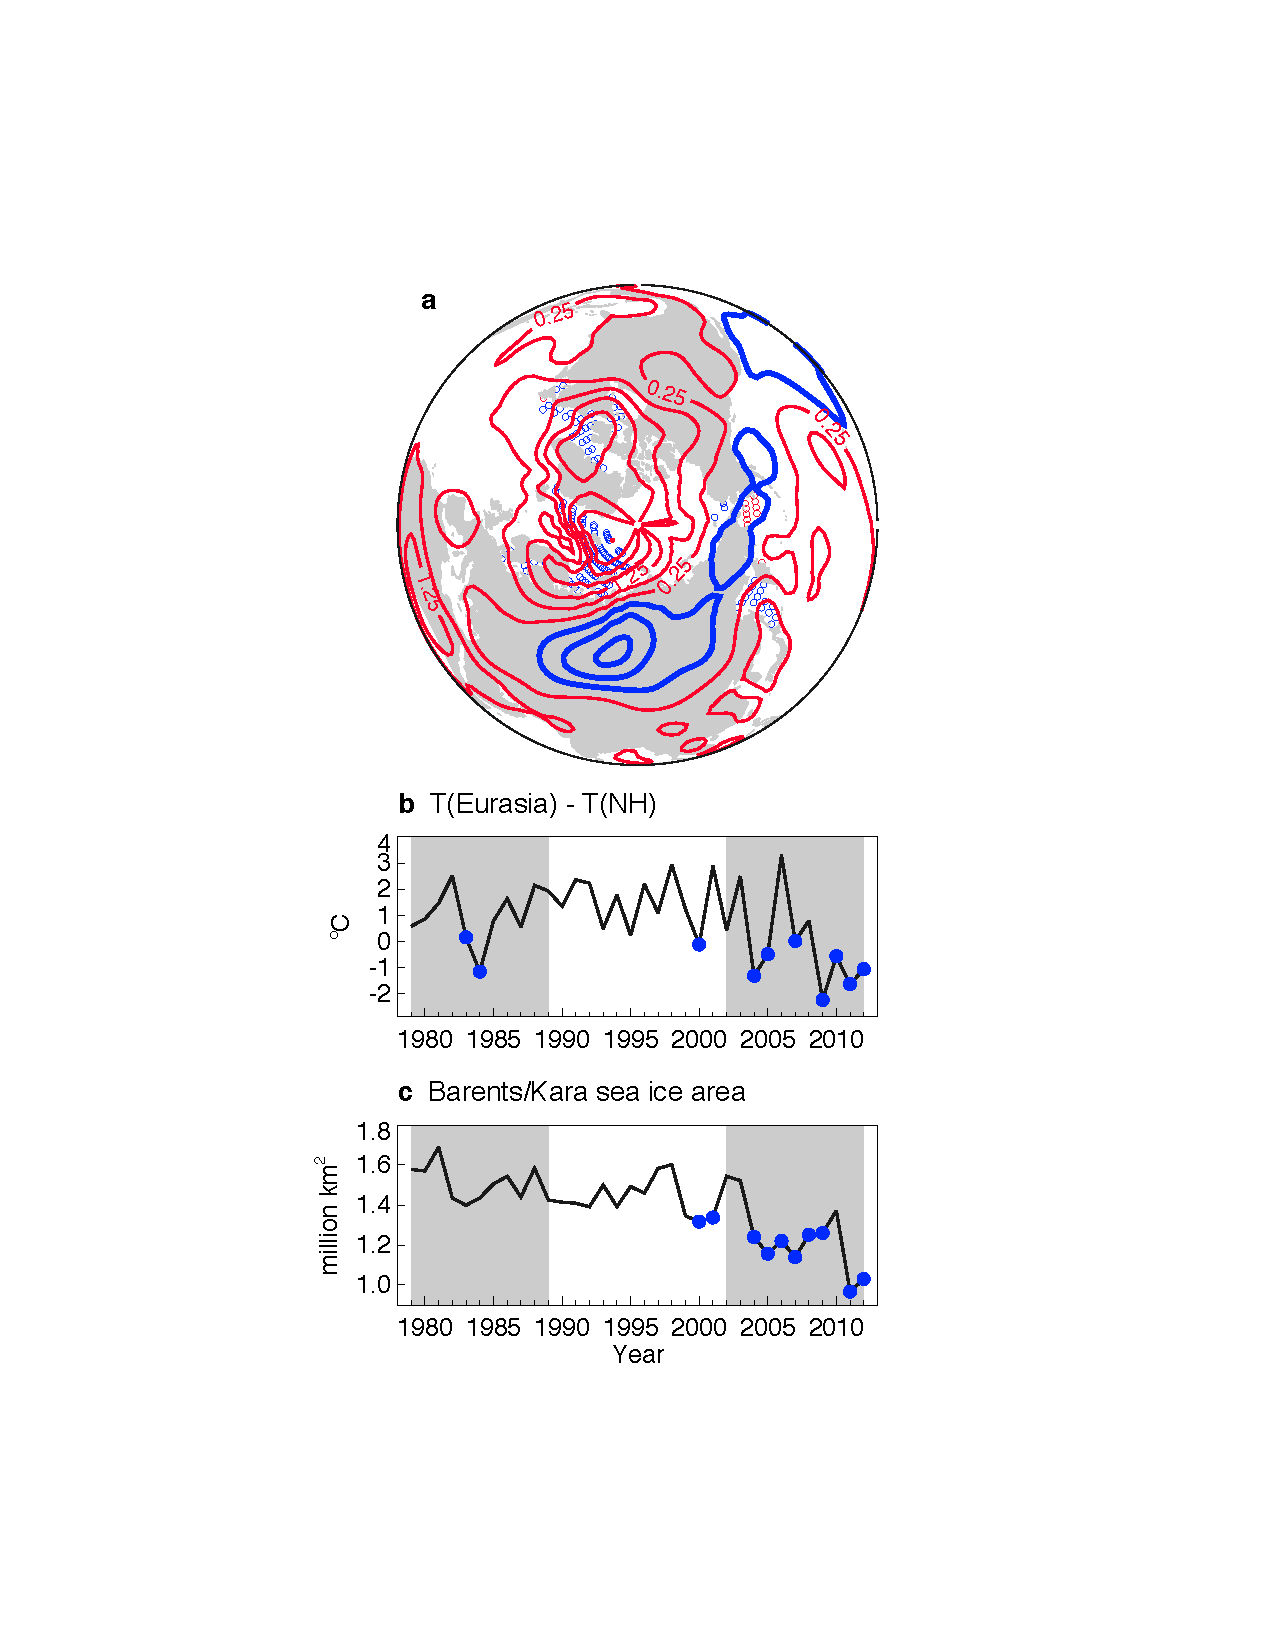
\includegraphics[width=20pc]{Word/Figure_1.pdf}
\caption{\textbf{Observed boreal winter SAT and SIC} a.) Map of GISTEMP winter surface air temperature anomalies as (2002-12) minus (1979-89) in contours. Contour interval is 0.5$^\circ$C with zero contour omitted. Stippling indicates regions of sea ice loss (blue) and gain (red) that are greater than 40\% in absolute terms. b.) Time series of Eurasian-averaged (35$^\circ$N - 60$^\circ$N, 40$^\circ$E - 120$^\circ$E) winter SAT with hemispheric (NH) winter temperature removed. Blue markers indicate the 10 most negative anomalies since 1979. c.) Time series of Barents-Kara Seas region (65$^\circ$N - 80$^\circ$N, 27$^\circ$E - 96$^\circ$E) winter sea ice area. Blue markers indicate the 10 lowest concentrations since 1979.
}
\label{fig:fig1} 
\end{figure}

\begin{figure}%[htbp] % the star afterwards makes it a one column fig in a 2-col document
\centering
\noindent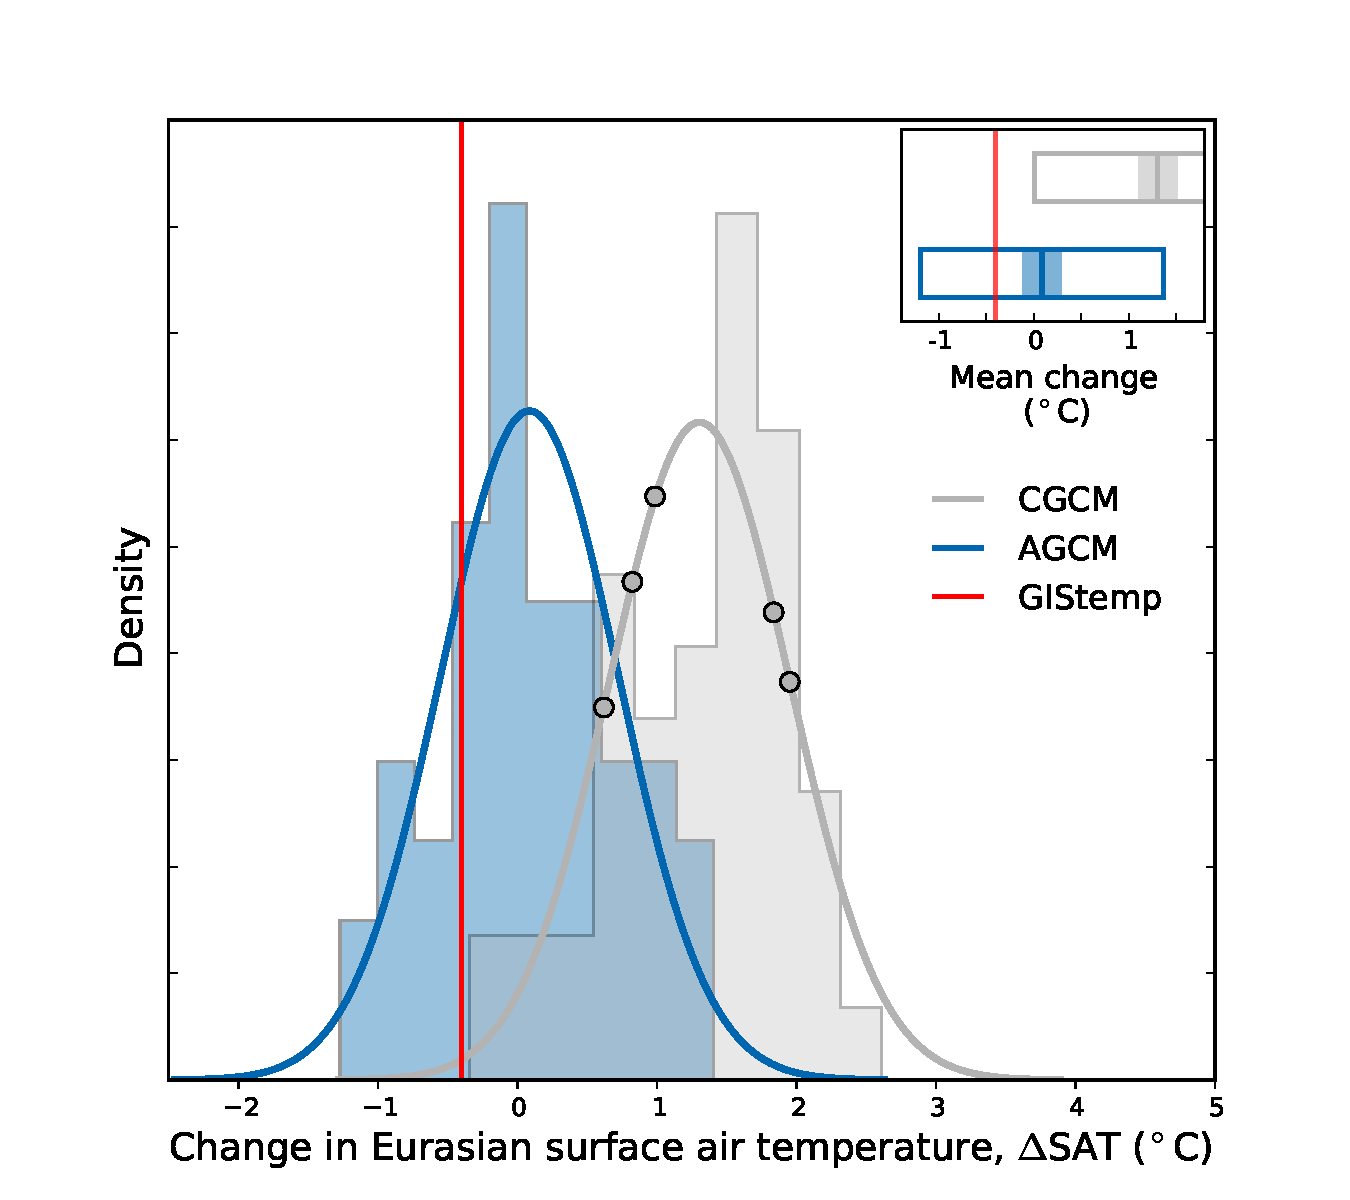
\includegraphics[width=39pc]{Word/Figure_2.pdf}
\caption{\textbf{Boreal winter Barents/Kara SIC and Eurasian SAT anomalies in CGCM.} a.) Histogram and associated probability distribution of DJF SIC (\%) anomalies (2002-12 minus 1979-89) averaged in the Barents/Kara Seas from CGCM (gray). The red vertical line shows the observed anomaly computed from the National Sea Ice Data Center (NSIDC) bootstrap dataset. Gray circles indicate the Barents/Kara Seas SIC anomalies in the 5 simulations whose Arctic sea ice concentration is used as boundary conditions to AGCM. Box at top shows the probability distribution mean (line), 2.5-97.5\% confidence range on the mean (shading), and 2.5-97.5\% range of the probability distribution (box). b.) is as a. but showing DJF Eurasian SAT anomalies ($^\circ$C). The red vertical line shows the observed anomaly computed from GISTEMP. Gray circles indicate the Eurasian SAT anomalies in the 5 simulations whose Arctic sea ice concentration is used as boundary conditions to AGCM. 
} % @@@ add: Filled markers indicate the present day period (2002-12) is significantly different from the past (1979-89) at the 90\% level using the Student’s T test of difference between two means. @@ Check confidence range: is it actually 2.5 - 97.5?
\label{fig:fig2} 
\end{figure}

\begin{figure}%[htbp] % the star afterwards makes it a one column fig in a 2-col document
\centering
\noindent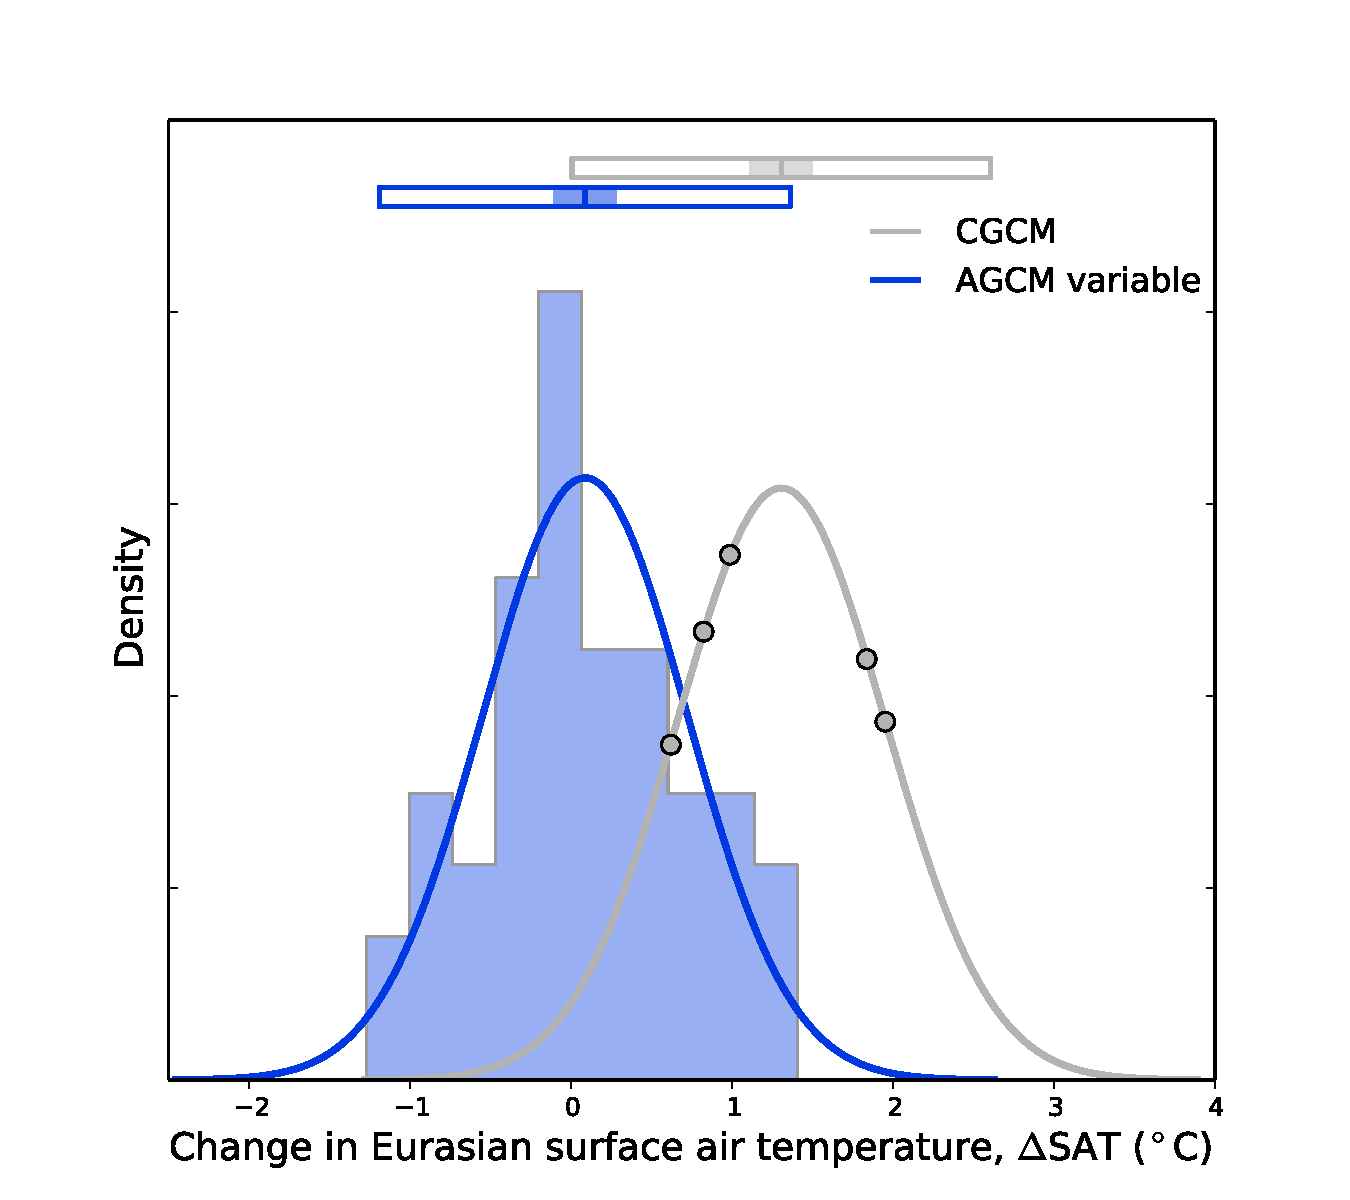
\includegraphics[width=20pc]{Word/Figure_3.pdf}
\caption{\textbf{Boreal winter Eurasian SAT anomalies in CGCM and AGCM.} Histogram and associated probability density distribution of AGCM winter Eurasian SAT ($^\circ$C) anomalies (blue). Probability density distribution of CGCM (gray) Eurasian SAT anomalies repeated from Figure \ref{fig:fig2} for comparison. Gray circles indicate the Eurasian SAT anomalies in the 5 simulations whose Arctic sea ice concentration is used as boundary conditions to AGCM. Boxes at top show the probability density distribution mean (line), 2.5-97.5\% confidence range on the mean (shading), and 2.5-97.5\% range of the probability density distribution (box).
} % @@@ add: Filled markers indicate the present day period (2002-12) is significantly different from the past (1979-89) at the 90\% level using the Student’s T test of difference between two means. @@ Check confidence range: is it actually 2.5 - 97.5?
\label{fig:fig3} 
\end{figure}

\begin{figure}%[htbp] % the star afterwards makes it a one column fig in a 2-col document
\centering
\noindent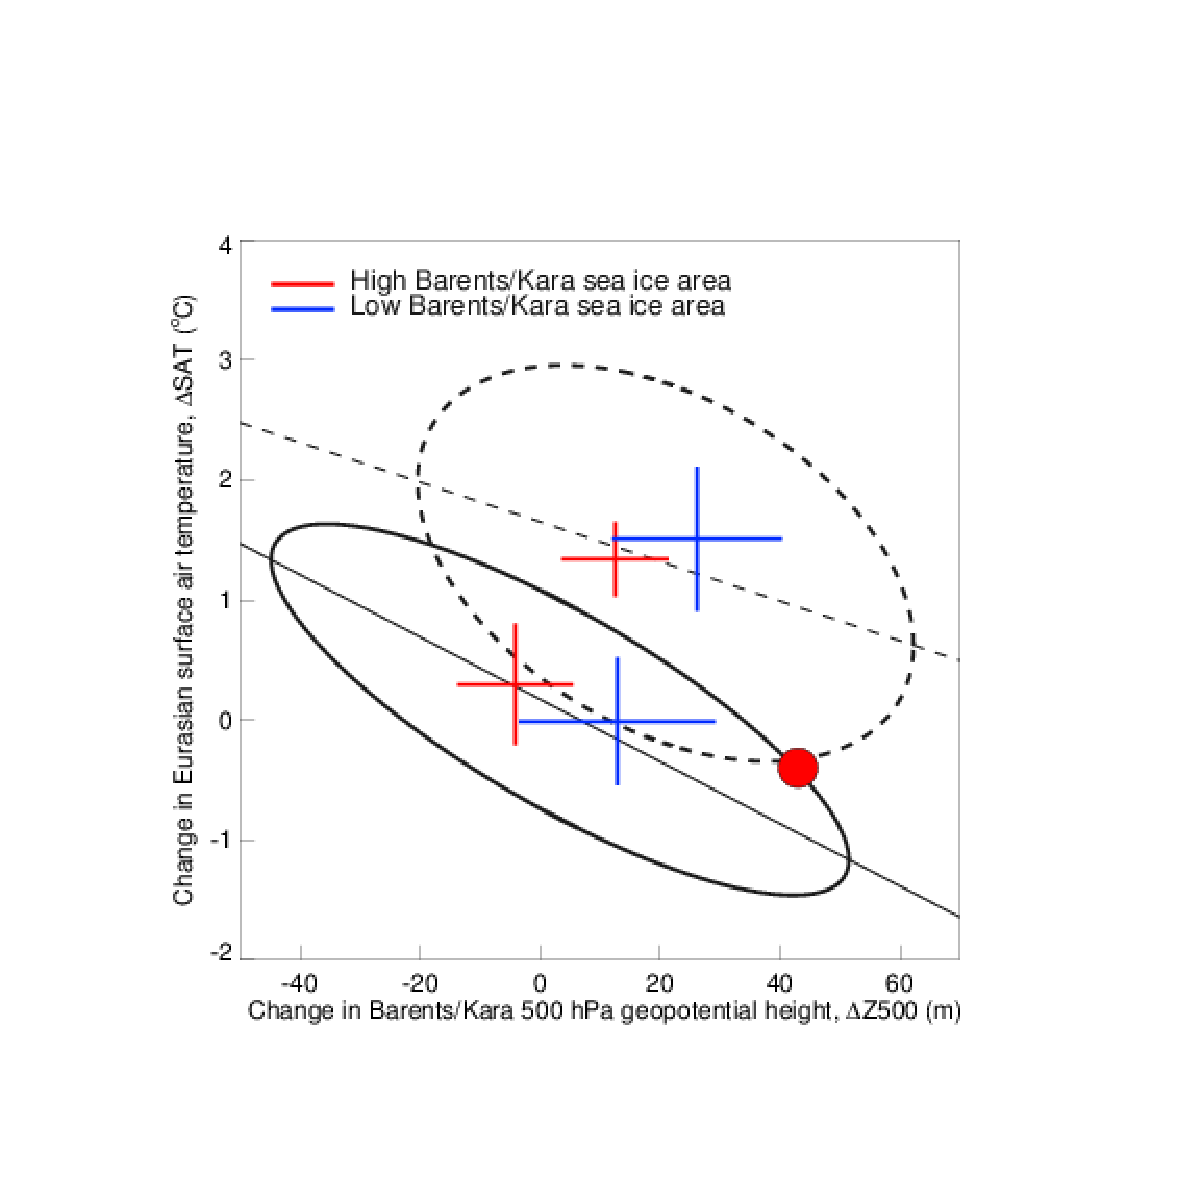
\includegraphics[width=20pc]{Word/Figure_4.pdf}
\caption{\textbf{Boreal winter Barents/Kara Z500 anomalies versus Eurasian SAT anomalies.} Ellipses depict the 2.5-97.5\% confidence range of the relationship between anomalies in Z500 averaged over the Barents/Kara Seas (m) and anomalies in Eurasian SAT ($^\circ$C) in CGCM (gray), AGCM\_variable (blue solid), and AGCM\_fixed (blue dashed), with associated linear regression lines. The red circle indicates the observed value from ERA-Interim and GISTEMP for Z500 and SAT, respectively. 
} %Plus markers show the value composited on the 10 smallest sea ice loss anomalies (red) and 10 largest sea ice loss anomalies (blue) in each ensemble. For both CGCM and AGCM, Barents/Kara Z500 composite anomalies are statistically different at the 95\% level (@@), but Eurasian SAT composite anomalies are not. @@ADD 10-samp avg of NSIDC simulation?
\label{fig:fig4} 
\end{figure}

\begin{figure}%[htbp] % the star afterwards makes it a one column fig in a 2-col document
\centering
\noindent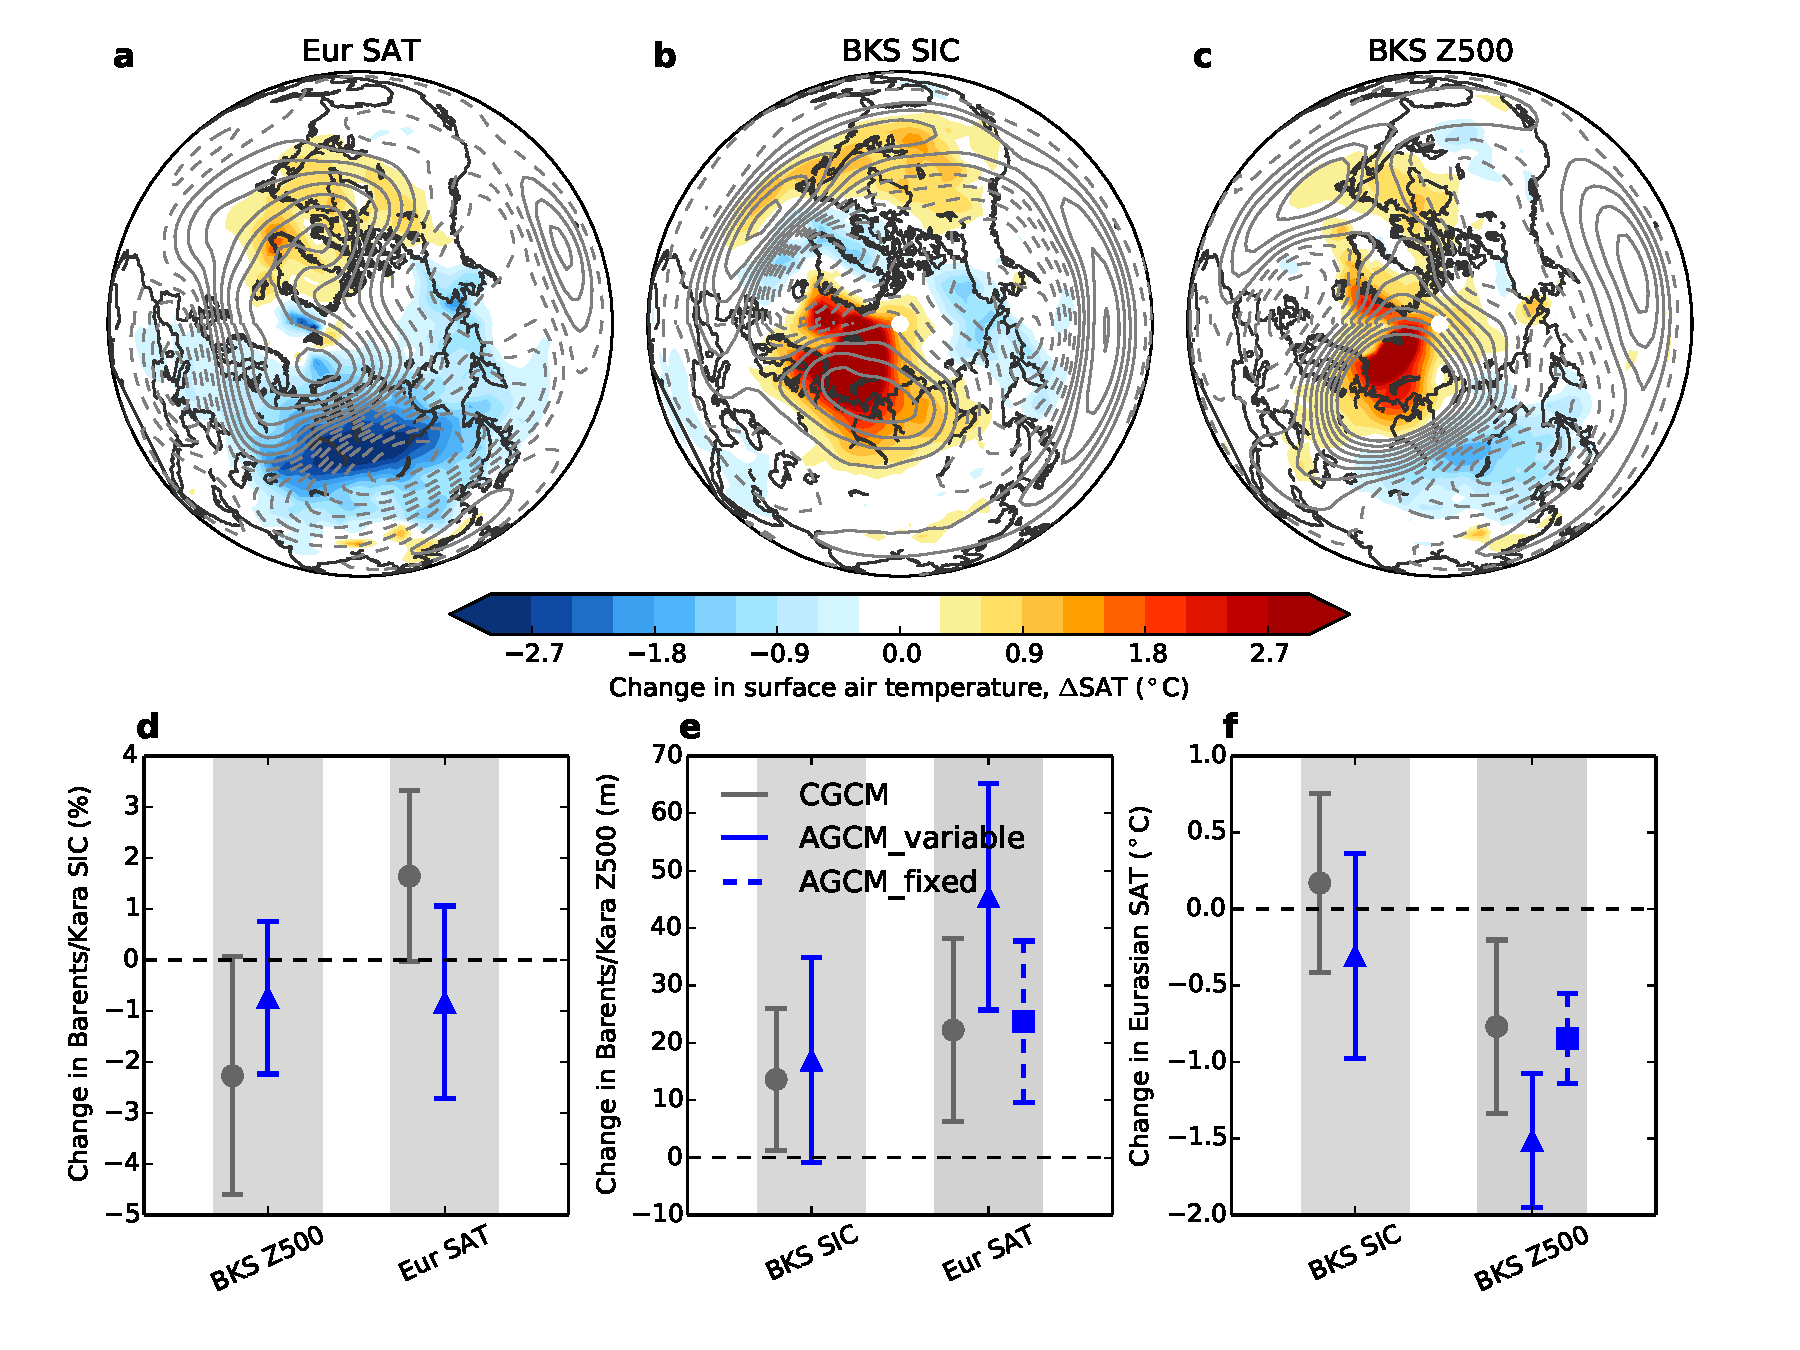
\includegraphics[width=39pc]{Word/Figure_5.pdf}
\caption{\textbf{Winter composites on Eurasian SAT, Barents/Kara SIC, and Barents/Kara Z500.} Spatial patterns of change in SAT (shading) and Z500 (contours) in CGCM associated with the a) `cold-warm' composite of Eur SAT, b) `low-high' composite of BKS SIC, and c) `high-low' composite of BKS Z500. Z500 contour interval is 4 m starting at +/- 2 m (no zero contour). d-f) show regional average anomalies and 2.5-97.5\% confidence ranges associated with the 3 composites shown in a-c. d) The change in SIC in the Barents/Kara Seas (\%) associated with the `high-low' composite of BKS Z500 (left column; map shown in c.) and associated with the `cold-warm' composite of Eur SAT (right column; map shown in a.) for CGCM (gray) and AGCM\_variable (blue solid). e) and f) are as d) but include AGCM\_fixed where defined (blue dashed), and show the change in Z500 (m) averaged over the Barents/Kara Seas and change in Eurasian SAT ($^\circ$C), respectively. Panels d-f only show anomalies for composites on a field other than itself. 
} %change in SAT ($^\circ$C) averaged over Eurasia (35$^\circ$N - 60$^\circ$N, 40$^\circ$E - 120$^\circ$E) associated with the `low-high' composite of BKS SIC (left column; map shown in a.), and associated with the `high-low' composite of BKS Z500 (right column; map shown in c.) for CGCM and AGCM. e) and f) are as d) but showing the change in SIC in the Barents/Kara Seas (\%) and change in Z500 (m) averaged over the Barents/Kara seas, respectively, and only show anomalies for composites on fields other than itself.
\label{fig:fig5} 
\end{figure}

% ==================== supp ===========
\begin{figure}%[htbp] % the star afterwards makes it a one column fig in a 2-col document
\centering
\noindent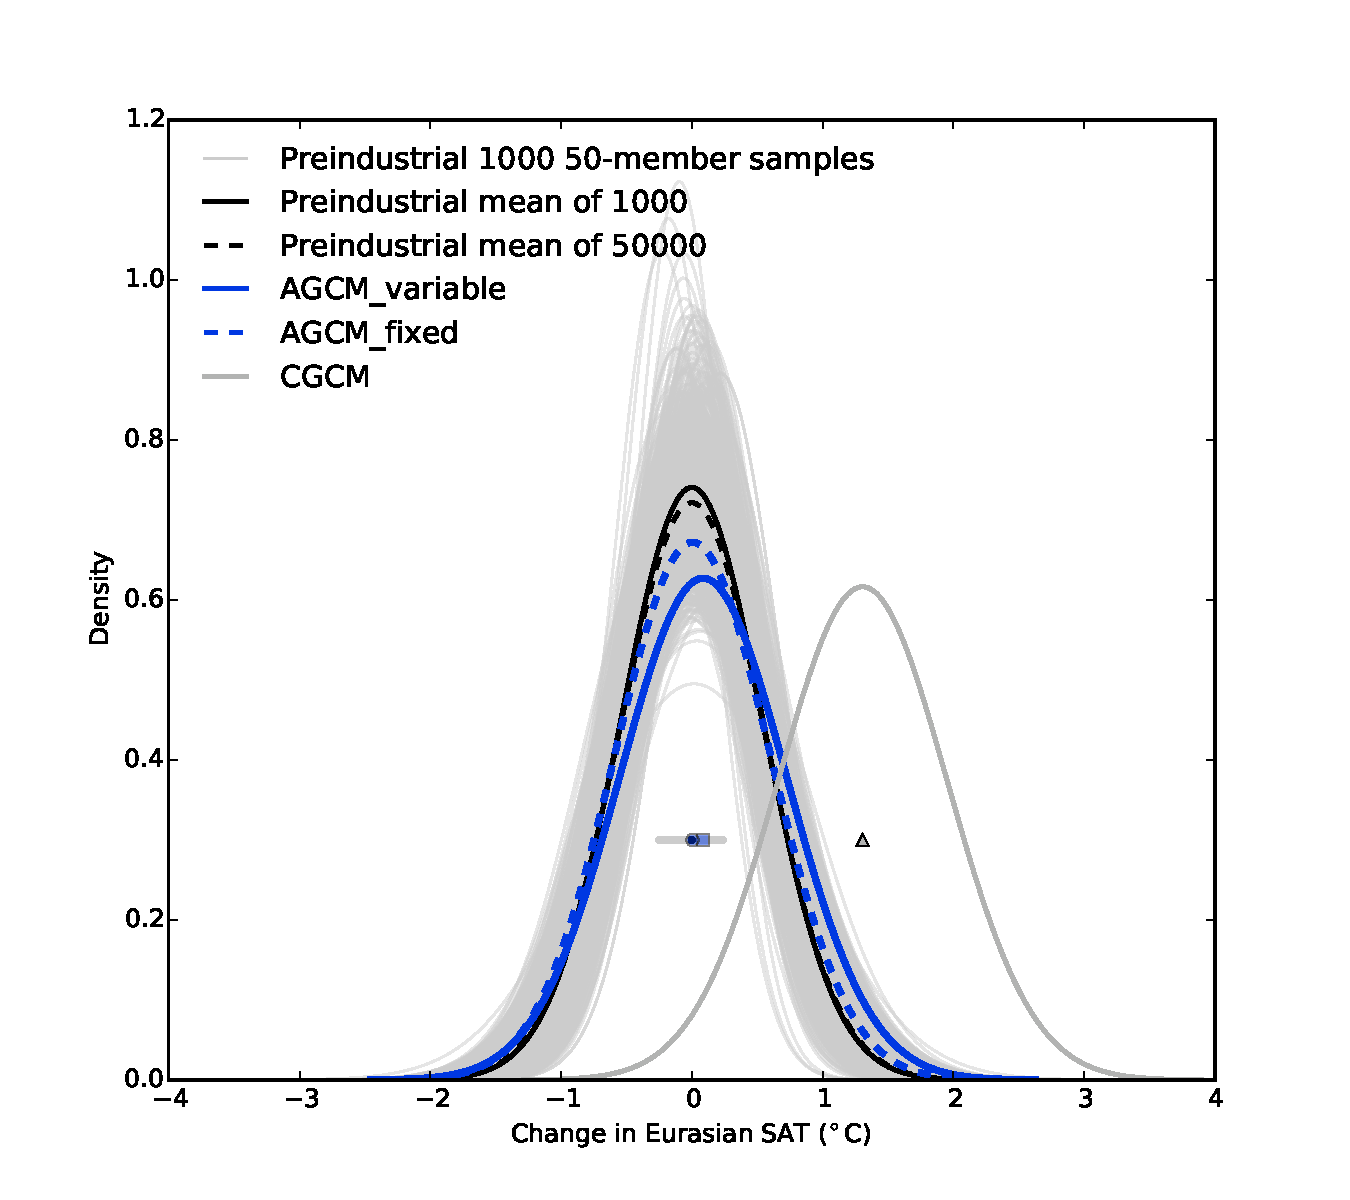
\includegraphics[width=29pc]{Word/SuppFigure_1_PIuncertainty.pdf}
\caption{\textbf{SUPPLEMENTARY S1: Boreal winter Eurasian SAT anomalies in CGCM, AGCM, and Preindustrial ensembles.} Probability density distributions (pdd) estimated from 50 DJF Eurasian SAT anomalies ($^\circ$C) sampled from the long Preindustrial simulation (see Methods) 1,000 times (thin gray) to estimate the sampling uncertainty of a 50-member distribution. Gray diamond markers show the means of the 1,000 pdd. The solid black curve shows the average of the 1,000 pdd, while dashed black shows the pdd estimated from the full 50,000 Preindustrial samples together. Black marker (hidden by blue circle marker) shows the mean of the solid black curve. Also shown are AGCM\_variable (blue solid; repeated from Figure 3 in the main text), AGCM\_fixed (blue dashed), and CGCM (thick gray; repeated from Figures 2 and 3 in the main text). Their pdd means are shown as markers (blue square, blue circle, and gray triangle for AGCM\_variable, AGCM\_fixed, and CGCM, respectively).
}
\label{fig:supp1} 
\end{figure}

\begin{figure}%[htbp] % the star afterwards makes it a one column fig in a 2-col document
\centering
\noindent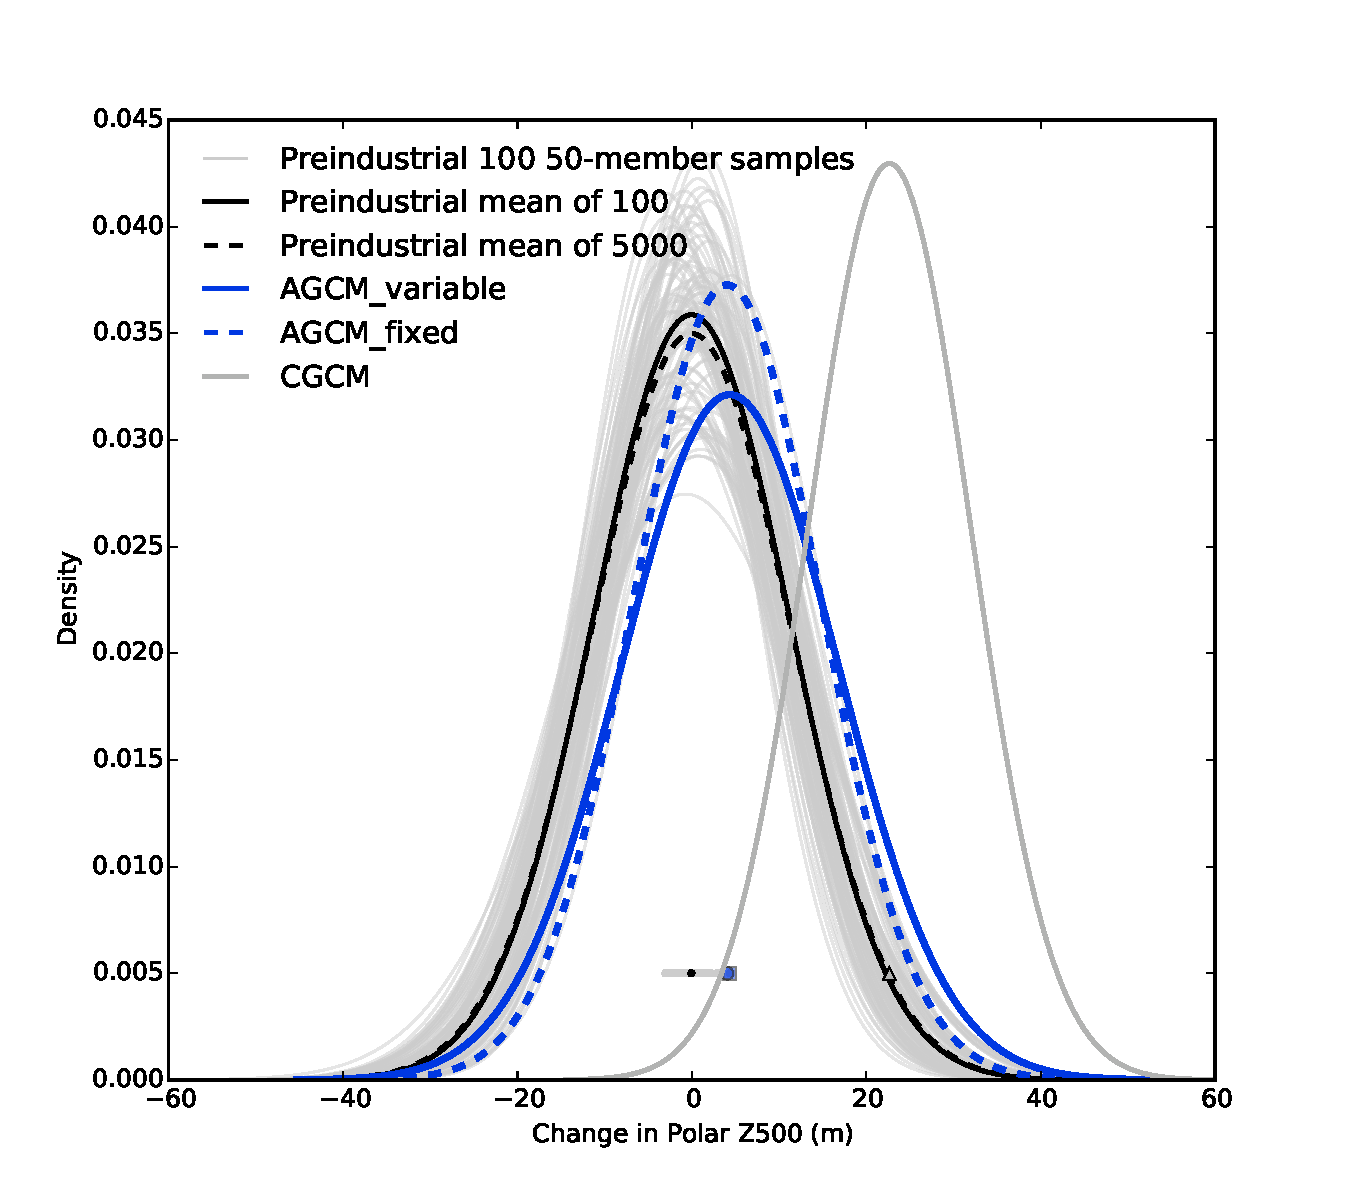
\includegraphics[width=29pc]{Word/SuppFigure_2_polarcapz500.pdf}
\caption{\textbf{SUPPLEMENTARY S2: Boreal winter polar cap Z500 anomalies in CGCM, AGCM, and Preindustrial ensembles.} As Figure S1 except showing DJF Z500 anomalies averaged north of 60$^\circ$N.
}
\label{fig:supp1} 
\end{figure}


\begin{figure}%[htbp] % the star afterwards makes it a one column fig in a 2-col document
\centering
\noindent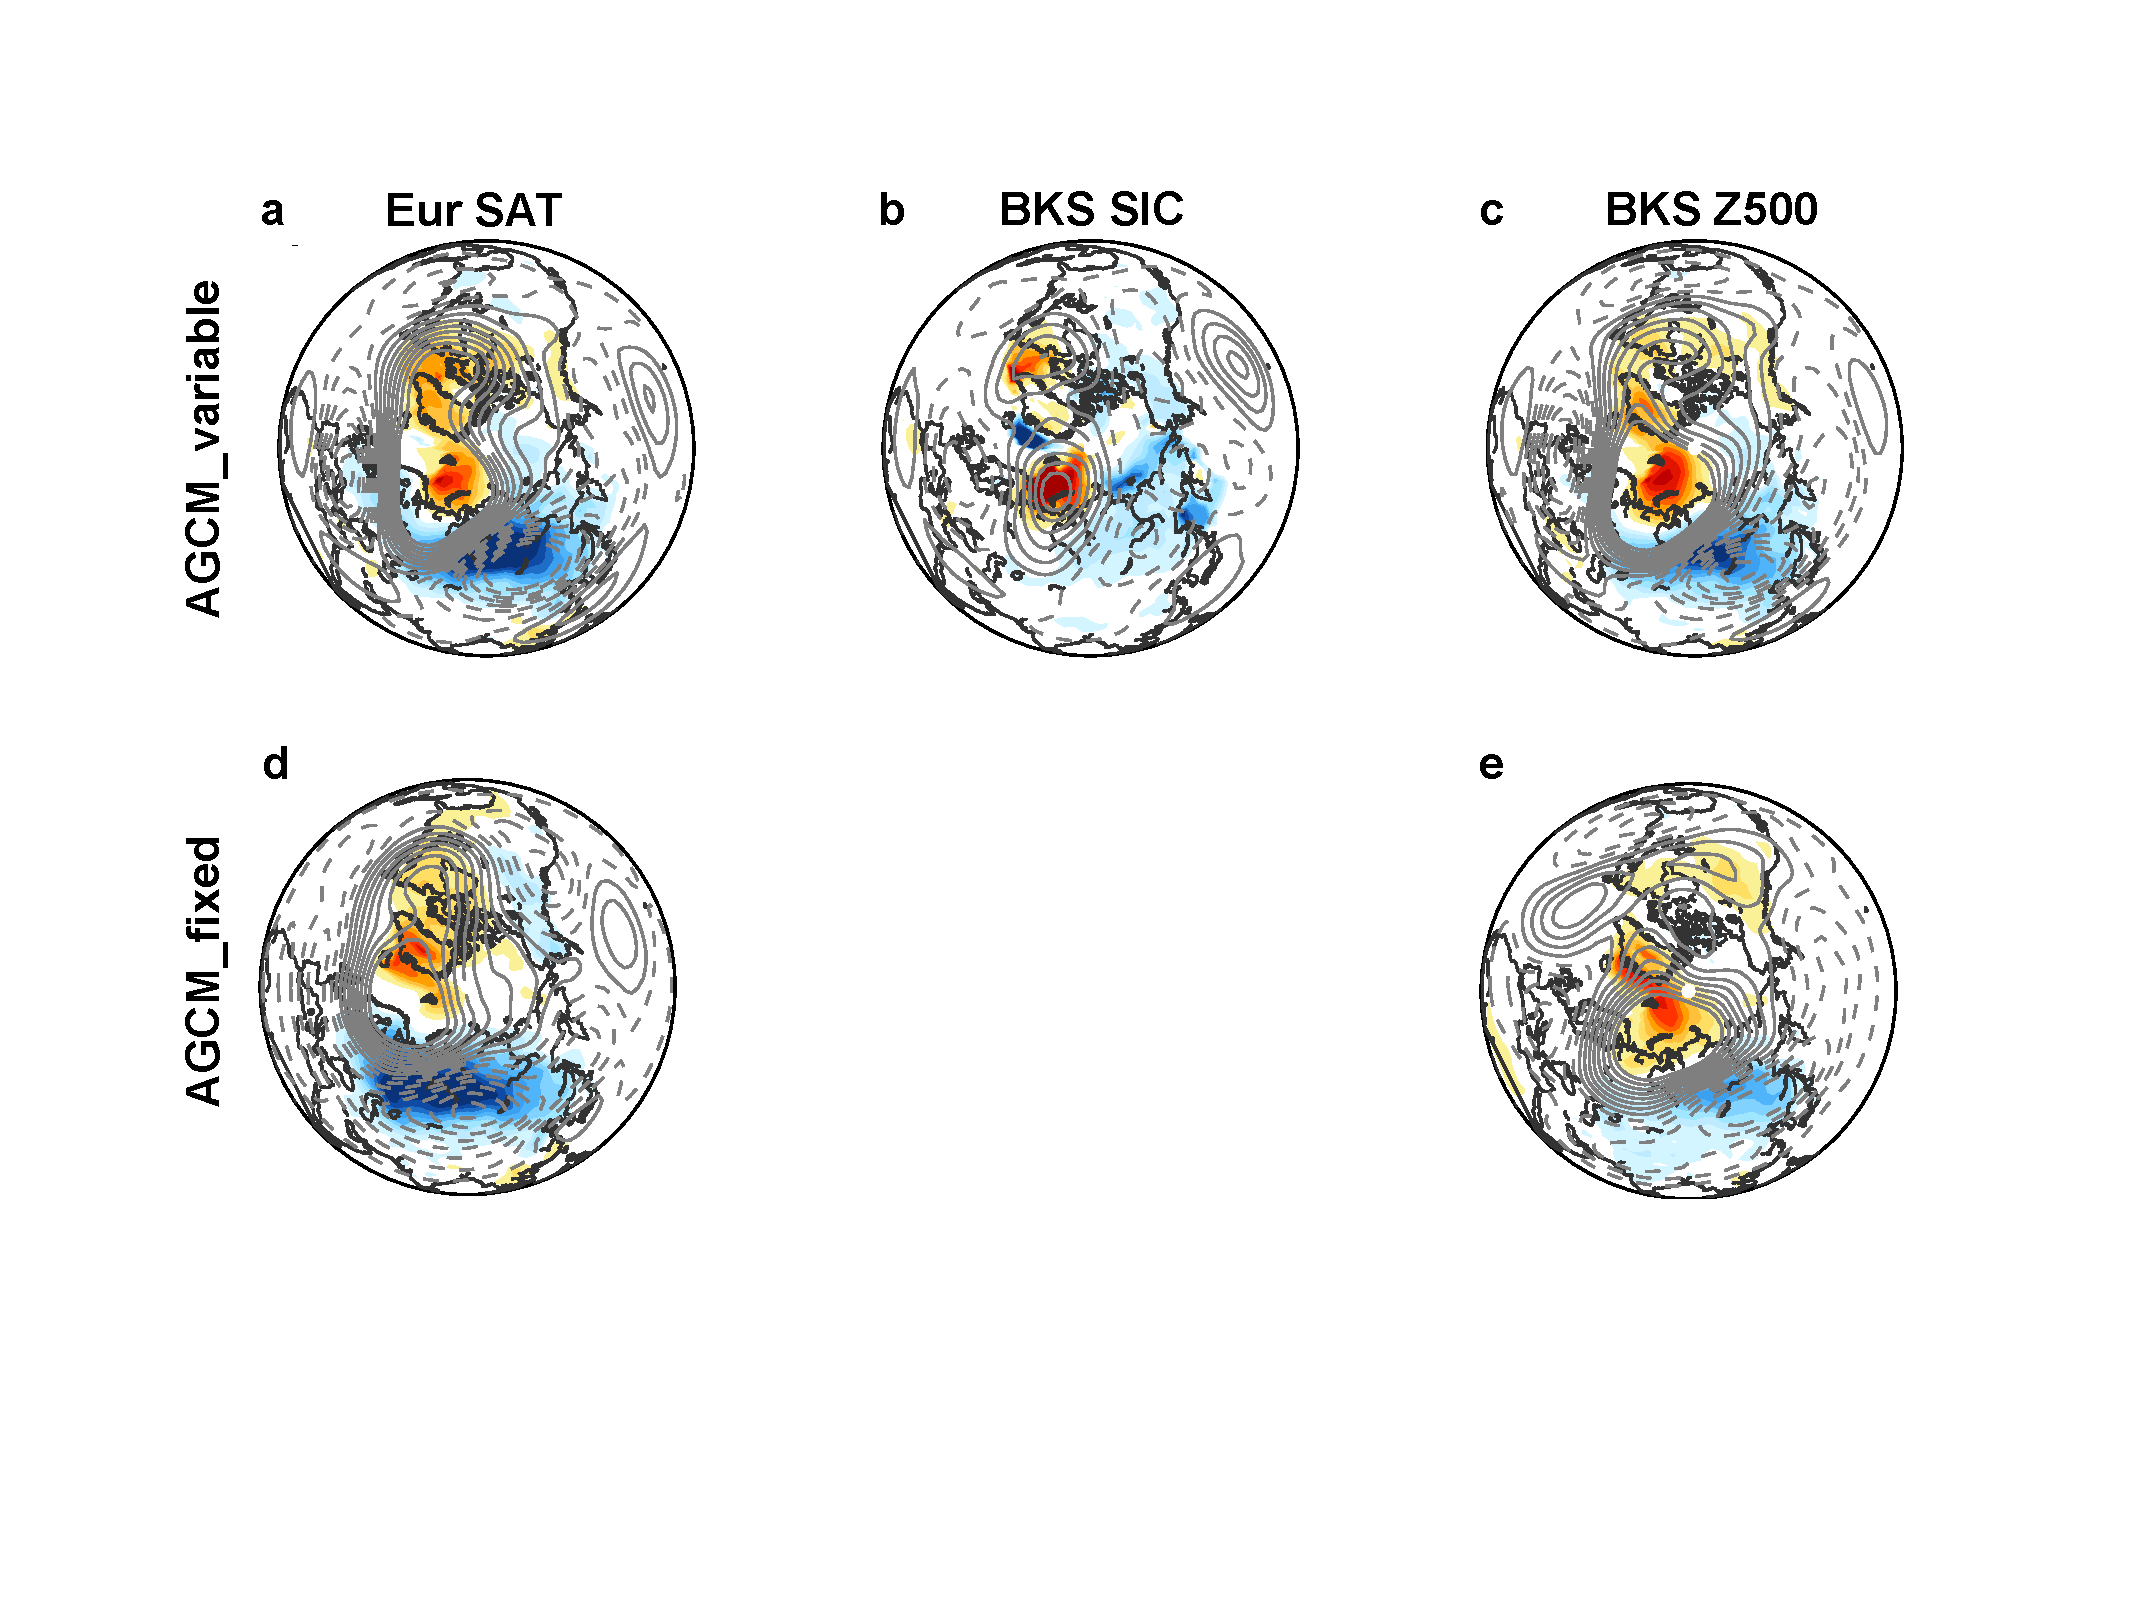
\includegraphics[width=39pc]{Word/SuppFig_xx.pdf}
\caption{\textbf{SUPPLEMENTARY S3: Winter composites on Eurasian SAT, Barents/Kara SIC, and Barents/Kara Z500.}  Spatial patterns of change in SAT (shading) and Z500 (contours) in AGCM\_variable associated with the a) `cold-warm' composite of Eur SAT, b) `low-high' composite of BKS SIC, and c) `high-low' composite of BKS Z500. Z500 contour interval is 4 m starting at +/- 2 m (no zero contour). d-e) are as a and c but for AGCM\_fixed where BKS SIC is not defined. %@@say something about same results with different regional avg
} 
\label{fig:supp3} 
\end{figure}

%\begin{figure}%[htbp] % the star afterwards makes it a one column fig in a 2-col document
%\centering
%\noindent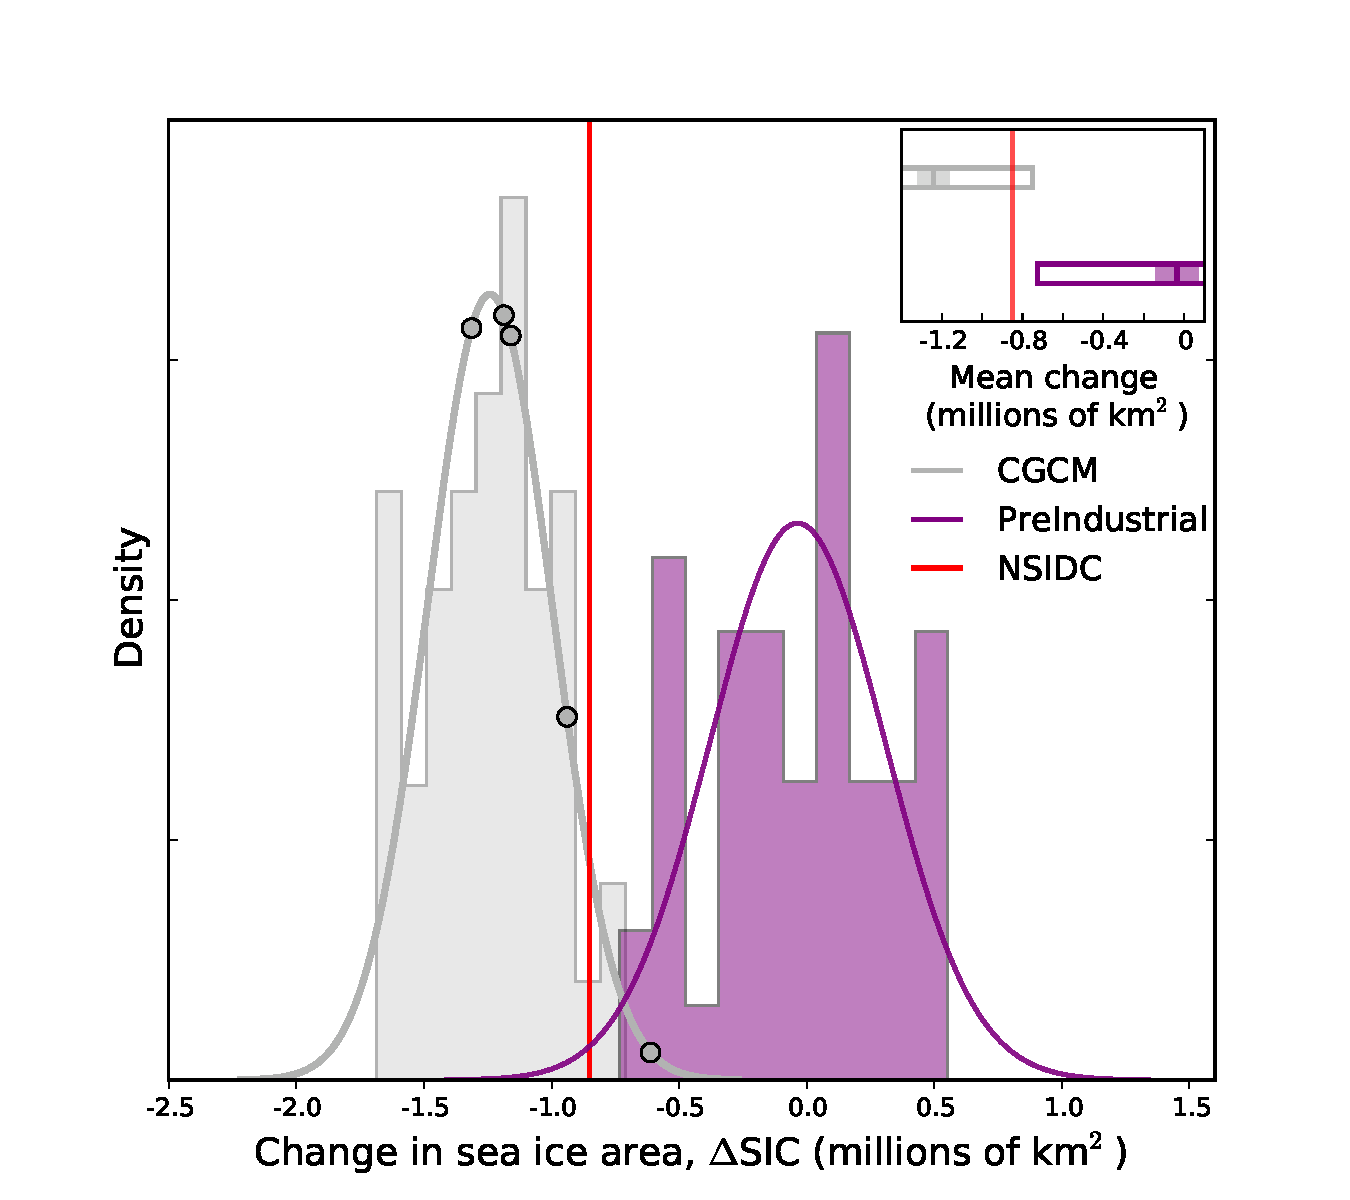
\includegraphics[width=39pc]{Word/SuppFig_1.pdf}
%\caption{\textbf{Winter Arctic sea ice area (SIA) anomalies.} Histograms and associated probability distributions of winter Arctic SIA anomalies (2002-12 minus 1979-89) sampled from the CGCM ensemble (gray) and anomalies sampled from the Preindustrial ensemble (purple). The red vertical line shows the observed anomaly computed from the National Sea Ice Data Center (NSIDC) bootstrap dataset. Gray circles indicate the Arctic SIA anomalies in the 5 simulations whose Arctic sea ice concentration is used as boundary conditions to the AGCM ensemble. The inset is as the main panel but shows the probability distribution mean (line), 5-95\% confidence range on the mean (shading), and 5-95\% range of the probability distribution (box).
%} 
%\label{fig:supfig1} 
%\end{figure}

%% Put the bibliography here, most people will use BiBTeX in
%% which case the environment below should be replaced with
%% the \bibliography{} command.

%\begin{thebibliography}{1}
%\end{thebibliography}
\newpage

%\bibliographystyle{ametsoc}
\bibliography{allrefs}





% ~/bibtexrefs/allrefs  == this is version controlled now, but will have to just copy into current dir?


%% Here is the endmatter stuff: Supplementary Info, etc.
%% Use \item's to separate, default label is "Acknowledgements"

\begin{addendum}
\item[Acknowledgements] 
\item[Author Contributions] 
 \item[Competing Interests] The authors declare that they have no competing financial interests.
\item[Correspondence] Correspondence and requests for materials should be addressed to K.E.M.~(email: kemccusk@uvic.ca).
\end{addendum}

%%
%% TABLES
%%
%% If there are any tables, put them here.
%%

\end{document}
